% Analytical Engine simulator project: https://www.cs.tcd.ie/Glenn.Strong/3d5/project1.pdf
\chapter{Machines}\label{ch:machines}

\chapquotew{It is unworthy of excellent people to lose hours like slaves in the labor of calculation which could safely be relegated to anyone else if machines were used.}{Gottfried Wilhelm von Leibniz, 1685}{10cm}\index{people}{Leibniz, Gottfried}

%\chapquotew{Well let's be clear right from the start, I never have been interested in computing, and I'm still not interested in computing. What I'm interested in is computers. I'm an engineer, I define the computer right from square one as a device which was designed to facilitate the performance of mathematics, the greater part of which would be very much better not done.}{F. C. Williams, engineer of the first stored-program computer}{10.75cm}\index{people}{Williams, F. C.}

\begin{exercisenote}
\exercisesonly{
\begin{center}
{\em Solutions for Chapter 6 provided by Ervin Varga.}
\end{center}
}
\end{exercisenote}

\begin{schemeregion}

%\begin{profile}
%Gottfried Wilhelm von Leibnitz 
%\end{profile}

The first five chapters focused on ways to use language to describe procedures.  Although finding ways to describe procedures succinctly and precisely would be worthwhile even if we did not have machines to carry out those procedures, the tremendous practical value we gain from being able to describe procedures comes from the ability of computers to carry out those procedures astoundingly quickly, reliably, and inexpensively.  As a very rough approximation, a typical laptop gives an individual computing power comparable to having every living human on the planet working for you without ever making a mistake or needing a break.

This chapter introduces computing machines.  Computers are different from other machines in two key ways: 
\begin{enumtight}
\item Whereas other machines amplify or extend our \emph{physical} abilities, computers amplify and extend our \emph{mental} abilities.
\item Whereas other machines are designed for a few specific tasks, computers can be \emph{programmed} to perform many tasks.  The simple computer model introduced in this chapter can perform \emph{all} possible computations.
\end{enumtight}

The next section gives a brief history of computing machines, from prehistoric calculating aids to the design of the first universal computers.  Section~\ref{sec:logic} explains how machines can implement logic.  Section~\ref{sec:modeling} introduces a simple abstract model of a computing machine that is powerful enough to carry out any algorithm.

We provide only a very shallow introduction to how machines can implement computations.  Our primary goal is not to convey the details of how to design and build an efficient computing machine (although that is certainly a worthy goal that is often pursued in later computing courses), but to gain sufficient understanding of the properties nearly all conceivable computing machines share to be able to predict properties about the costs involved in carrying out a particular procedure.  The following chapters use this to reason about the costs of various procedures.  In Chapter~\ref{ch:computability}, we use it to reason about the range of problems that can and cannot be solved by any mechanical computing machine.

\section{History of Computing Machines}\label{sec:computing-machines}\index{general}{computing machines}

The goal of early machines was to carry out some physical process with less effort than would be required by a human.  These machines took physical things as inputs, performed physical actions on those things, and produced some physical output.  For instance, a cotton gin takes as input raw cotton, mechanically separates the cotton seed and lint, and produces the separated products as output.  

The first big leap toward computing machines was the development of machines whose purpose is abstract rather than physical.  Instead of producing physical things, these machines used physical things to {\em represent} information.  The output of the machine is valuable because it can be interpreted as information, not for its direct physical effect.

\index{general}{counting}Our first example is not a machine, but using fingers to count.  The base ten number system used by most human cultures reflects using our ten fingers for counting.\footnote{Not all human cultures use base ten number systems.  For example, many cultures including the Maya and Basque adopted base twenty systems counting both fingers and toes.  This was natural in warm areas, where typical footwear left the toes uncovered.}  Successful shepherds needed to find ways to count higher than ten.  Shepherds used stones to represent numbers, making the cognitive leap of using a physical stone to represent some quantity of sheep.  A shepherd would count sheep by holding stones in his hand that represent the number of sheep.
%%\sidepicture{0.35}{images/Inca_Quipu.jpg}{Inca Khipu}{} %http://en.wikipedia.org/wiki/Image:Inca_Quipu.jpg

More complex societies required more counting and more advanced calculating.  The Inca civilization in Peru used knots in collections of strings known as {\em khipu}
to keep track of thousands of items for a hierarchical system of taxation.\cut{Different kinds of knots at different position on different strings could be used to represent thousands of different numbers.}\index{general}{khipu}\index{general}{abacus} Many cultures developed forms of abaci, including the ancient Mesopotamians and Romans.  An {\em abacus} performs calculations by moving beads on rods.  The Chinese {\em suan pan} (``calculating plate'') \sidepicture{0.75}{images/Boulier1.jpg}{Suan Pan}{} %http://en.wikipedia.org/wiki/Image:Boulier1.JPG
is an abacus with a beam subdividing the rods, typically with two beads above the bar (each representing 5), and five beads below the beam (each representing 1).  An operator can perform addition, subtraction, multiplication, and division by following mechanical processes using an abacus.

All of these machines require humans to move parts to perform calculations.  As machine technology improved, automatic calculating machines were built where the operator only needed to set up the inputs and then turn a crank or use some external power source to perform the calculation.  \cut{The first known automatic calculating machine was built in Germany by Wilhelm Schickard in 1623.\marginquote{What you have done by calculation I have just tried to do by way of mechanics. I have conceived a machine consisting of eleven complete and six incomplete sprocket wheels; it calculates instantaneously and automatically from given numbers, as it adds, subtracts, multiplies and divides.}{Wilhelm Schickard, letter to Johannes Kepler, 1623}\cut{and could perform addition and subtraction mechanically, and multiplication and division with assistance from the operator. Other than as a historical artifact, however, Schickard's machine had little impact and the only machine burned in 1624.}\index{people}{Schickard, Wilhelm}
}
% . Image from David Monniaux.
% source: http://en.wikipedia.org/wiki/Image:Arts_et_Metiers_Pascaline_dsc03869.jpg
\index{people}{Pascal, Blaise}\index{general}{Pascaline}The first automatic calculating machine to be widely demonstrated was the {\em Pascaline}, \sidepicture{0.08}{images/800px-Arts_et_Metiers_Pascaline_dsc03869.jpg}{Pascaline}{David Monniaux} built by then nineteen-year old French mathematician Blaise Pascal (also responsible for Pascal's triangle from Exploration 5.1\LATER{\ref{excur:pascal}}) to replace the tedious calculations he had to do to manage his father's accounts.  The Pascaline had five wheels, each representing one digit of a number, linked by gears to perform addition with carries.  %http://en.wikipedia.org/wiki/File:Arts_et_Metiers_Pascaline_dsc03869.jpg
Gottfried Wilhelm von Leibniz built the first machine capable of performing all four basic arithmetic operations (addition, subtraction, multiplication, and division) fully mechanically in 1694.\index{people}{Leibniz, Gottfried}

Over the following centuries, more sophisticated mechanical calculating machines were developed but these machines could still only perform one operation at a time.  Performing a series of calculations was a tedious and error-prone process in which a human operator had to set up the machine for each arithmetic operation, record the result, and reset the machine for the next calculation.

\index{general}{programmability}The big breakthrough was the conceptual leap of programmability.  A machine is \emph{programmable} if its inputs not only control the values it operates on, but the operations it performs.  
%http://images.google.com/hosted/life/l?q=charles+babbage&prev=/images%3Fq%3Dcharles%2Bbabbage%26imgsz%3Dxxlarge%26um%3D1%26hl%3Den%26client%3Dfirefox-a%26rls%3Dorg.mozilla:en-US:official%26sa%3DN&imgurl=19fc9fba4ea4a1cb

The first programmable computing machine was envisioned (but never successfully built) in the 1830s by Charles Babbage.%\sidepicture{0.42}{images/charlesbabbage.jpg}{Charles Babbage}{Life Magazine}
\index{people}{Babbage, Charles} % need permission 
Babbage was born in London in 1791 and studied mathematics at Cambridge.  In the 1800s, calculations were done by looking up values in large books of mathematical and astronomical tables.  These tables were computed by hand, and often contained errors.  \cut{Babbage and astronomer John Herschel examined one set of tables in 1821 and found it contained thousands of errors. } The calculations were especially important for astronomical navigation, and when the values were incorrect a ship would miscalculate its position at sea (sometimes with tragic consequences).  

\sidequote{We got nothing for our $\pounds$17,000 but Mr. Babbage's grumblings. We should at least have had a clever toy for our money.}
{Richard~Sheepshanks, \emph{Letter to the Board of Visitors of the Greenwich Royal Observatory},~1854}
Babbage sought to develop a machine to mechanize the calculations to compute these tables.  Starting in 1822, he designed a steam-powered machine known as the Difference Engine to compute polynomials needed for astronomical calculations using Newton's method of successive differences\index{people}{Newton, Isaac} (a generalization of Heron's method from Exploration~\ref{exploration:sqrt}).  
The Difference Engine was never fully completed. but led Babbage to envision a more general calculating machine.\cut{despite receiving funding from the Royal Astronomical Society responsible for producing the astronomical navigation tables, Babbage endured repeated difficulty securing continued funding.}

This new machine, the Analytical Engine, designed between 1833 and 1844, was the first general-purpose computer envisioned.  It was designed so that it could be programmed to perform any calculation.  One breakthrough in Babbage's design was to feed the machine's outputs back into its inputs.  This meant the engine could perform calculations with an arbitrary number of steps by cycling outputs back through the machine. 

The Analytical Engine was programmed using punch cards, based on the cards that were used by Jacquard looms.   Each card could describe an instruction such as loading a number into a variable in the store, moving values, performing arithmetic operations on the values in the store, and, most interestingly, jumping forward and backwards in the instruction cards.  \sidepicture{0.16}{images/analytical-engine.jpg}{Analytical Engine}{Science Museum, London}
The Analytical Engine supported conditional jumps where the jump would be taken depending on the state of a lever in the machine (this is essentially a simple form of the if expression). 
%\sidepicture{0.4}{images/jacquard-loom-cards.jpg}{Jacquard loom cards}{} %http://en.wikipedia.org/wiki/File:Jacquard.loom.cards.jpg

In 1842, Charles Babbage visited Italy and described the Analytical Engine to Luigi Menabrea, an Italian engineer, military officer, and mathematician who would later become Prime Minister of Italy.  Menabrea published a description of Babbage's lectures in French.  \index{people}{Ada, Countess of Lovelace}Ada Augusta Byron King (also known as Ada, Countess of Lovelace) translated the article into English.  

In addition to the translation, Ada added a series of notes to the article.  The notes included a program to compute Bernoulli numbers, the first detailed program for the Analytical Engine.  Ada was the first to realize the importance and interest in creating the programs themselves, and envisioned how programs could be used to do much more than just calculate mathematical functions.  This was the first computer program ever described, and Ada is recognized as the first computer programmer.
\sidepicture{0.36}{images/Ada_Lovelace.jpg}{Ada}{} 

%http://en.wikipedia.org/wiki/File:Ada_Lovelace.jpg
Despite Babbage's design, and Ada's vision, the Analytical Engine was never completed.  It is unclear whether the main reason for the failure to build a working Analytical Engine was due to limitations of the mechanical components available at the time, or due to Babbage's inability to work with his engineer collaborator or to secure continued funding.  

\marginquote{On two occasions I have been asked by members of Parliament, ``Pray, Mr. Babbage, if you put into the machine wrong figures, will the right answers come out?'' I am not able rightly to apprehend the kind of confusion of ideas that could provoke such a question.}{Charles Babbage} 
The first working programmable computers would not appear for nearly a hundred years.  Advances in electronics enabled more reliable and faster components than the mechanical components used by Babbage, and the desperation brought on by World War II spurred the funding and efforts that led to working general-purpose computing machines.  \LATER{We tell the story of one of those machines in 
Exploration~\ref{excur:colossus}.}  

% in Radio and the Electronic Engineer, 1975 http://www.turing.org.uk/turing/scrapbook/manmach.html
The remaining conceptual leap is to treat the program itself as data\cut{, analogous to how we use procedures as inputs and outputs in Chapter~\ref{ch:problems}}.  In Babbage's Analytical Engine, the program is a stack of cards and the data are numbers stored in the machine.  The machine cannot alter its own program.  

The idea of treating the program as just another kind of data the machine can process was developed in theory by Alan Turing in the 1930s (Section~\ref{sec:modeling} of this chapter describes his model of computing), and first implemented by the Manchester Small-Scale Experimental Machine (built by a team at Victoria University in Manchester) in 1948.  

%\sidequote{With this store available, the next step was to build a computer around it. Tom Kilburn and I knew nothing about computers, but a lot about circuits. Professor Newman and Mr A. M. Turing knew a lot about computers and substantially nothing about electronics. They took us by the hand and explained how numbers could live in houses with addresses and how if they did they could be kept track of during a calculation.}{F. C. Williams, engineer of the Manchester Small-Scale Experimental Machine} 
This computer (and all general-purpose computers in use today) stores the program itself in the machine's memory.  Thus, the computer can create new programs by writing into its own memory.  This power to change its own program is what makes stored-program computers so versatile.

\LATER{describe these machines?}

%\marginquote{The whole of the developments and operations of analysis are now capable of being executed by machinery. ... As soon as an Analytical Engine exists, it will necessarily guide the future course of science.}{Charles Babbage, \emph{Passages from the Life of a Philosopher}, 1864}

%\marginquote{Notwithstanding the numerous logarithmic tables which have since appeared, those of Mr. Babbage are still held in high esteem by all upon whom the laborious calculations of astronomy and mathematical science devolve.}{The Times, Obituary for Charles Babbage, October 23, 1871 (reprinted in \emph{Eminent Persons}, Volume 1)}
\beforeex
\begin{exercise}
Babbage's design for the Analytical Engine called for a store holding 1000 variables, each of which is a 50-digit (decimal) number.  How many bits could the store of Babbage's Analytical Engine hold? 
\solution{
With 50 decimal digits we can differentiate $10^{50}$ numbers covering the
range $[0, 10^{50} - 1]$.  Thus, we need $\ceil{\log_2 10^{50}} = 167$
bits per variable. Thus, The machine could store 167,000 bits in
total, which is 20,875 bytes (or approximately 20KB).
}
\end{exercise}
\afterex
 
\section{Mechanizing Logic}\label{sec:logic}

%\marginquote{\cut{That which renders Logic possible, is the existence in our minds of general notions---our ability to conceive of a class, and to designate its individual members by a common name.  The theory of Logic is thus intimately connected with that of Language.  }A successful attempt to express logical propositions by symbols, the laws of whose combinations should be founded upon the laws of the mental processes which they represent, would, so far, be a step toward a philosophical language.}{George Boole, {\em Mathematical Analysis of Logic}, 1847}

This section explains how machines can compute, starting with simple logical operations.  \index{general}{Boolean}We use \definition{Boolean logic}, in which there are two possible values: \true\ (often denoted as \bI), and \false\ (often denoted as \bO).  The Boolean datatype in Scheme is based on Boolean logic.  Boolean logic is named for George Boole\index{people}{Boole, George}, a self-taught British mathematician who published {\em An investigation into the Laws of Thought, on Which are founded the Mathematical Theories of Logic and Probabilities} in 1854.  Before Boole's work, logic focused on natural language discourse.  Boole made logic a formal language to which the tools of mathematics could be applied. 

We illustrate how logical functions can be implemented mechanically by describing some logical machines.  Modern computers use electrons to compute because they are small (more than a billion billion billion ($10^{31}$) electrons fit within the volume of a grain of sand), fast (approaching the speed of light), and cheap (more than a billion billion ($10^{22}$) electrons come out of a power outlet for less than a cent).  \sidepicture{0.10}{images/boole-1-1000.jpg}{George Boole}{} %http://www.mathematik.de/mde/information/kalenderblatt/logik/bilder/boole-1-1000.jpg % need permission for this
They are also invisible and behave in somewhat mysterious ways, however, so we will instead consider how to compute with wine (or your favorite colored liquid).  The basic notions of mechanical computation don't depend on the medium we use to compute, only on our ability to use it to represent values and to perform simple logical operations.

\subsection{Implementing Logic}

To implement logic using a machine, we need physical ways of representing the two possible values.  We use a full bottle of wine to represent \true\ and an empty bottle of wine to represent \false.  If the value of an input is \true, we pour a bottle of wine in the input nozzle; for \false\ inputs we do nothing.  Similarly, electronic computers typically use presence of voltage to represent \true, and absence of voltage to represent \false.  

\shortsection{And}  A logical \function{and} function takes two inputs and produces one output.  The output is \true\ if both of the inputs are \true; otherwise the output is \false.  We define a \scheme|logical-and| procedure using an if expression:\footnote{Scheme provides a special form \scheme|and| that performs the same function as the logical \function{and} function.  It is a special form, though, since the second input expression is not evaluated unless the first input expression evaluates to \true.}
\begin{schemedisplay}
(define (logical-and a b) (if a b false))
\end{schemedisplay}

To design a mechanical implementation of the logical \function{and} function, we want a simpler definition that does not involve implementing something as complex as an if expression.  

A different way to define a function is by using a table to show the corresponding output value for each possible pair of input values.  This approach is limited to functions with a small number of possible inputs; we could not define addition on integers this way, since there are infinitely many possible different numbers that could be used as inputs.  For functions in Boolean logic, there are only two possible values for each input (\true\ and \false) so it is feasible to list the outputs for all possible inputs.

We call a table defining a Boolean function a \definition{truth table}.  If there is one input, the table needs two entries, showing the output value for each possible input.  When there are two inputs, the table needs four entries, showing the output value for all possible combinations of the input values.  The truth table for the logical \function{and} function is:

\begin{center}
	\begin{tabular}{cc|c} % \hline
		%\multicolumn{2}{c|}{\bf Inputs} & \multicolumn{1}{c} {\bf Output} \\ \hline 
		\var{A} &  \var{B} & \scheme|(and A B)| \\ \hline
		\false & \false & \false \\
		\true & \false & \false \\
		\false & \true & \false \\
		\true & \true & \true \\ %\hline	
	\end{tabular}
\end{center}

We design a machine that implements the function described by the truth table: if both inputs are \true\ (represented by full bottles of wine in our machine), the output should be \true; if either input is \false, the output should be \false\ (an empty bottle).  One way to do this is shown in Figure~\ref{fig:wine-and-gate}.  Both inputs pour into a basin.  The output nozzle is placed at a height corresponding to one bottle of wine in the collection basin, so the output bottle will fill (representing \true), only if both inputs are true.

\begin{figure}[!htbp] 
\begin{center}
{\scalebox{0.3}{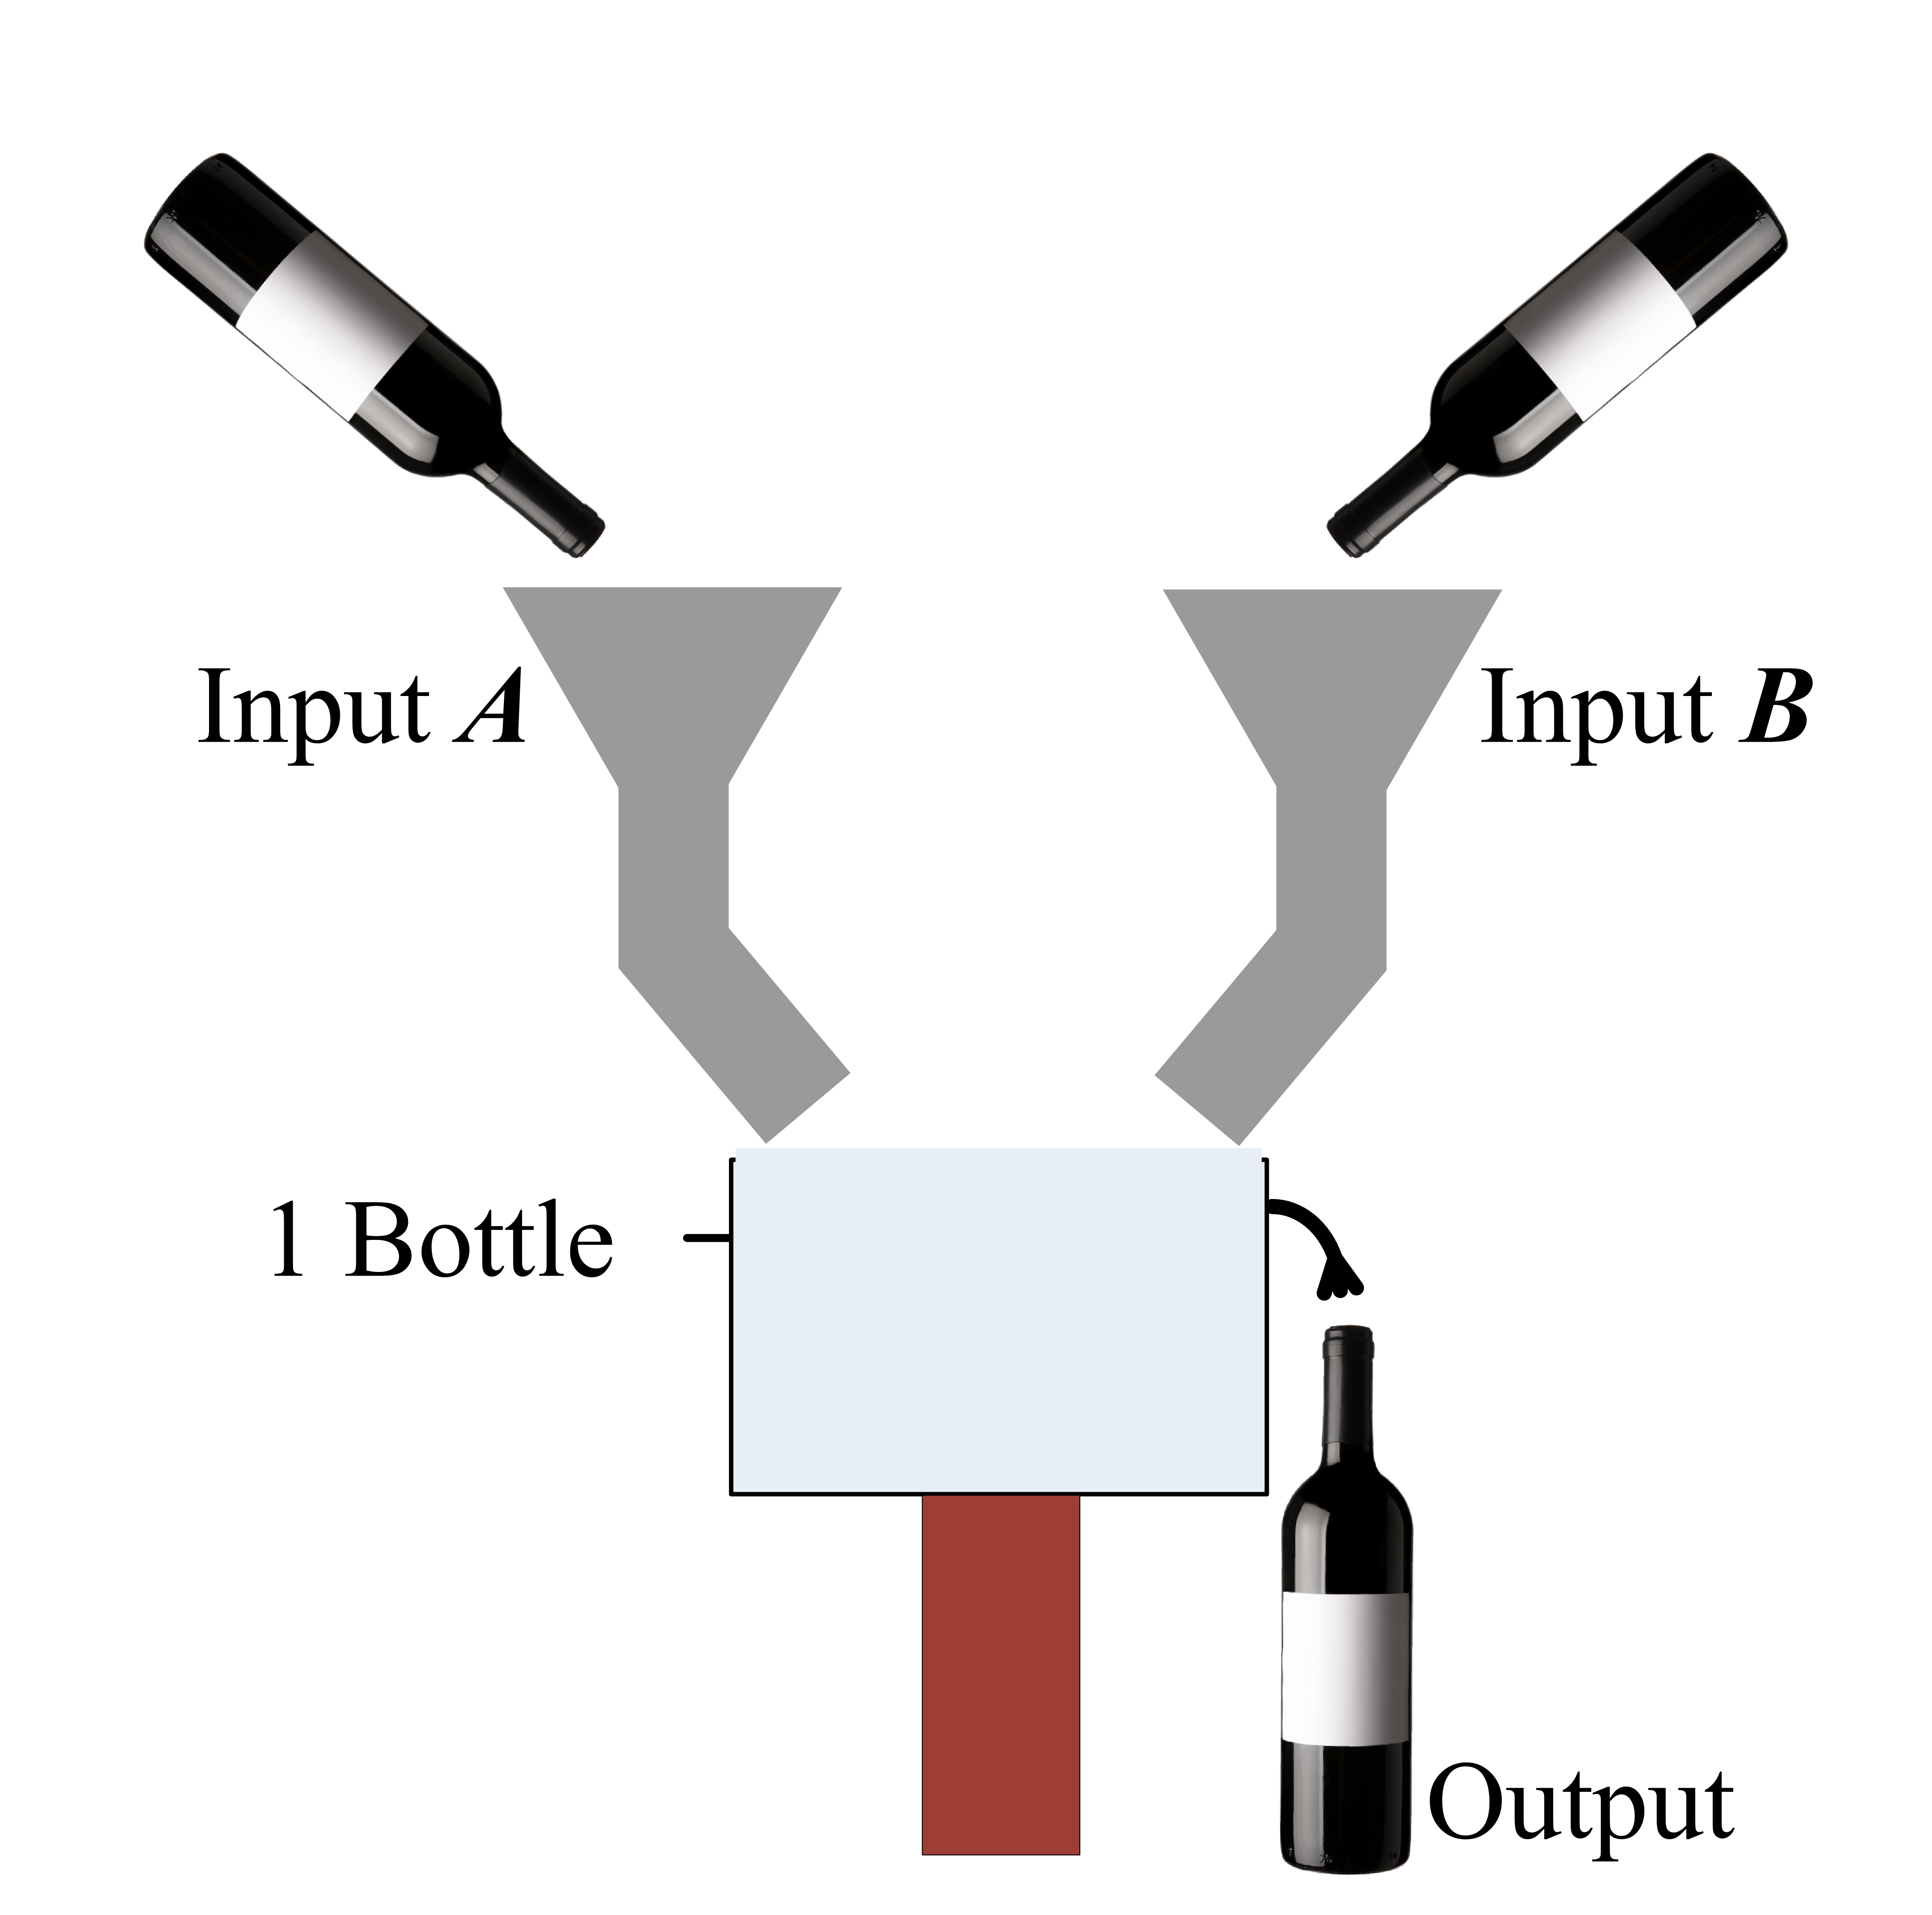
\includegraphics{figures/and-gate.png}}} 
\end{center}
\caption{Computing \function{and} with wine.\label{fig:wine-and-gate}}
\end{figure}

%\subsection{The Digital Abstraction}
The design in Figure~\ref{fig:wine-and-gate} would probably not work very well in practice.  Some of the wine is likely to spill, so even when both inputs are \true\ the output might not be a full bottle of wine.  What should a $\frac{3}{4}$ full bottle of wine represent?  What about a bottle that is half full?

The solution is the \definition{digital abstraction}.  Although there are many different quantities of wine that could be in a bottle, regardless of the actual quantity the value is interpreted as only one of two possible values: \true\ or \false.  If the bottle has more than a given threshold, say half full, it represents \true; otherwise, it represents \false.  This means an infinitely large set of possible values are abstracted as meaning \true, so it doesn't matter which of the values above half full it is.  

%This is dangerous, however, since when the bottle is close to $\frac{1}{2}$ full there is some chance the result would be interpreted as the wrong value.  Hence, we consider the middle range invalid.  For example, readings below $\frac{1}{4}$ represent \false, readings above $\frac{3}{4}$ represent \true, and readings between $\frac{1}{4}$ and $\frac{3}{4}$ are considered \emph{invalid} (that is, they do not represent either value with enough certainty to be considered valid).

The digital abstraction provides a transition between the continuous world of physical things and the logical world of discrete values.  It is much easier to design computing systems around discrete values than around continuous values; by mapping a range of possible continuous values to just two discrete values, we give up a lot of information but gain in simplicity and reliability.  Nearly all computing machines today operate on discrete values using the digital abstraction.  

\shortsection{Or} The logical \function{or} function takes two inputs, and outputs true if any of the inputs are true:\footnote{Scheme provides a special form \scheme|or| that implements the logical \scheme|or| function, similarly to the \scheme|and| special form.  If the first input evaluates to \schemeresult|true|, the second input is not evaluated and the value of the \scheme|or| expression is \schemeresult|true|.} 
\begin{center}
	\begin{tabular}{cc|c} 
		% \multicolumn{2}{|c|}{\bf Inputs} & {\bf Output} \\ 
		\var{A} & \var{B} & \scheme|(or A B)| \\ \hline
		\false & \false & \false \\
		\true & \false & \true \\
		\false & \true & \true \\
		\true & \true & \true \\ 
	\end{tabular}
\end{center}
Try to invent your own design for a machine that computes the \function{or} function before looking at one solution in Figure~\ref{fig:wine-or-gate}.

\shortsection{Implementing not} The output of the \function{not} function is the opposite of the value of its input:
\begin{center}
	\begin{tabular}{c|c} % \hline
		%{\bf Input} & {\bf Output} \\ 
		\var{A} & (\function{not} \var{A}) \\ \hline
		\false & \true \\
		\true & \false \\ % \hline	
	\end{tabular}
\end{center}

It is not possible to produce a logical \function{not} without some other source of wine; it needs to create wine (to represent \true) when there is none input (representing \false).  To implement the \function{not} function, we need the notion of a {\em source current} and a {\em clock}.  The source current injects a bottle of wine on each clock tick.  The clock ticks periodically, on each operation.  The inputs need to be set up before the clock tick.  When the clock ticks, a bottle of wine is sent through the source current, and the output is produced.  Figure~\ref{fig:wine-not-gate} shows one way to implement the \function{not} function.

\begin{figure}[ht]
\centering
\subfigure[Computing \function{or} with wine.]{
{\scalebox{0.25}{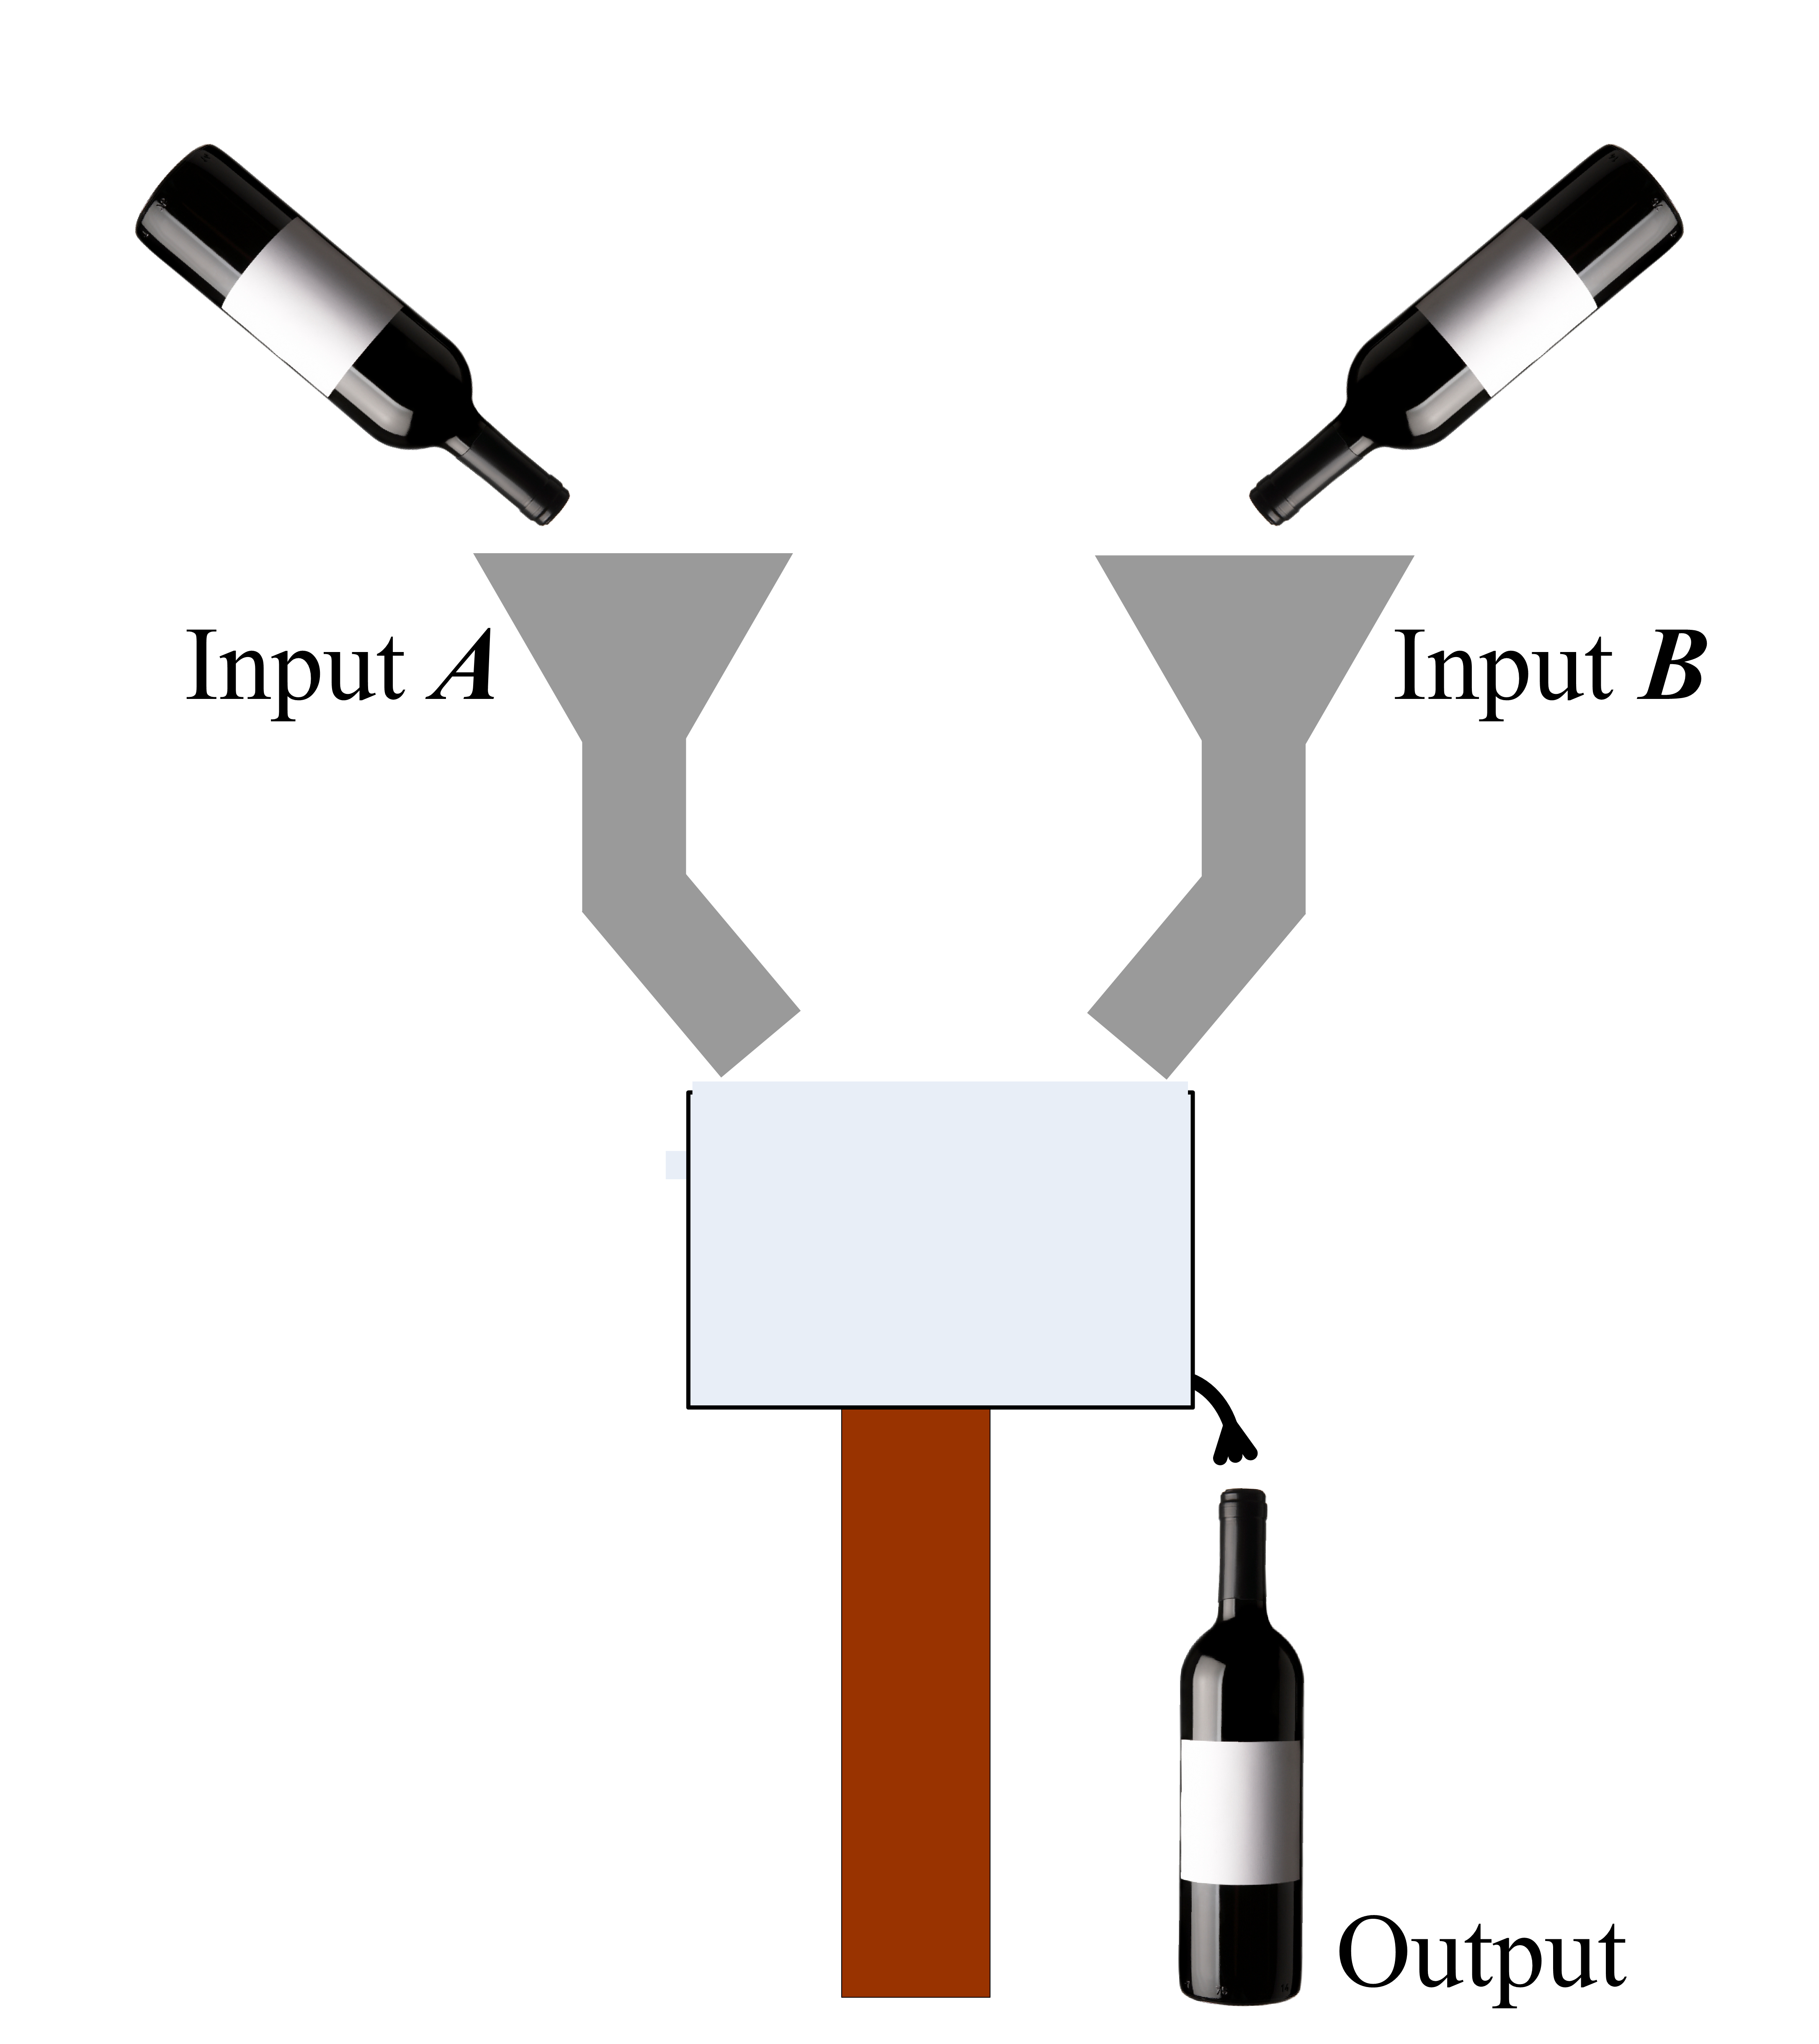
\includegraphics{figures/or-gate.png}}}\hspace{0.6cm} 
\label{fig:wine-or-gate}
}
\subfigure[Computing \function{not} with wine.]{
\hspace{0.6cm}{\scalebox{0.3}{\includegraphics{figures/not-gate.png}}} 
\label{fig:wine-not-gate}
}
\caption{Computing logical \function{or} and \function{not} with wine}
\subcapw{{\bf (a)} The \function{or} machine is similar to the \function{and} machine in design, except we move the output nozzle to the bottom of the basin, so if either input is \true, the output is \true; when both inputs are \true, some wine is spilled but the logical result is still \true.  

{\bf (b)} The \function{not} machine uses a clock.  Before the clock tick, the input is set.  If the input is \true, the float is lifted, blocking the source opening; if the input i \false, the float rests on the bottom of the basin.  When the clock ticks, the source wine is injected.  If the float is up (because of the \true\ input), the opening is blocked, and the output is empty (\false).  If the float is down (because of the \false\ input), the opening is open, the source wine will pour across the float, filling the output (representing \true).  (This design assumes wine coming from the source does not leak under the float, which might be hard to build in a real system.)

\vspace*{2ex}
}
\end{figure}

\subsection{Composing Operations}\label{sec:composingoperations}

We can implement \function{and}, \function{or} and \function{not} using wine, but is that enough to perform interesting computations? In this subsection, we consider how simple logical functions can be combined to implement any logical function; in the following subsection, we see how basic arithmetic operations can be built from logical functions.
  
We start by making a three-input conjunction function. The \function{and3} of three inputs is \true\ if and only if all three inputs are \true.  One way to make the three-input \function{and3} is to follow the same idea as the two-input \function{and} where all three inputs pour into the same basin, but make the basin with the output nozzle above the two bottle level. 

Another way to implement a three-input \function{and3} is to compose two of the two-input \function{and} functions, similarly to how we composed procedures in Section~\ref{sec:compose}.  Building \function{and3} by composing two two-input \function{and} functions allows us to construct a three-input \function{and3} without needing to design any new structures, as shown in Figure~\ref{fig:three-and-compose}.  The output of the first \function{and} function is fed into the second \function{and} function as its first input; the third input is fed directly into the second \function{and} function as its second input.  We could write this as \scheme|(and (and A B) C)|.

\begin{figure}[!bth]
\begin{center}
{\scalebox{0.25}{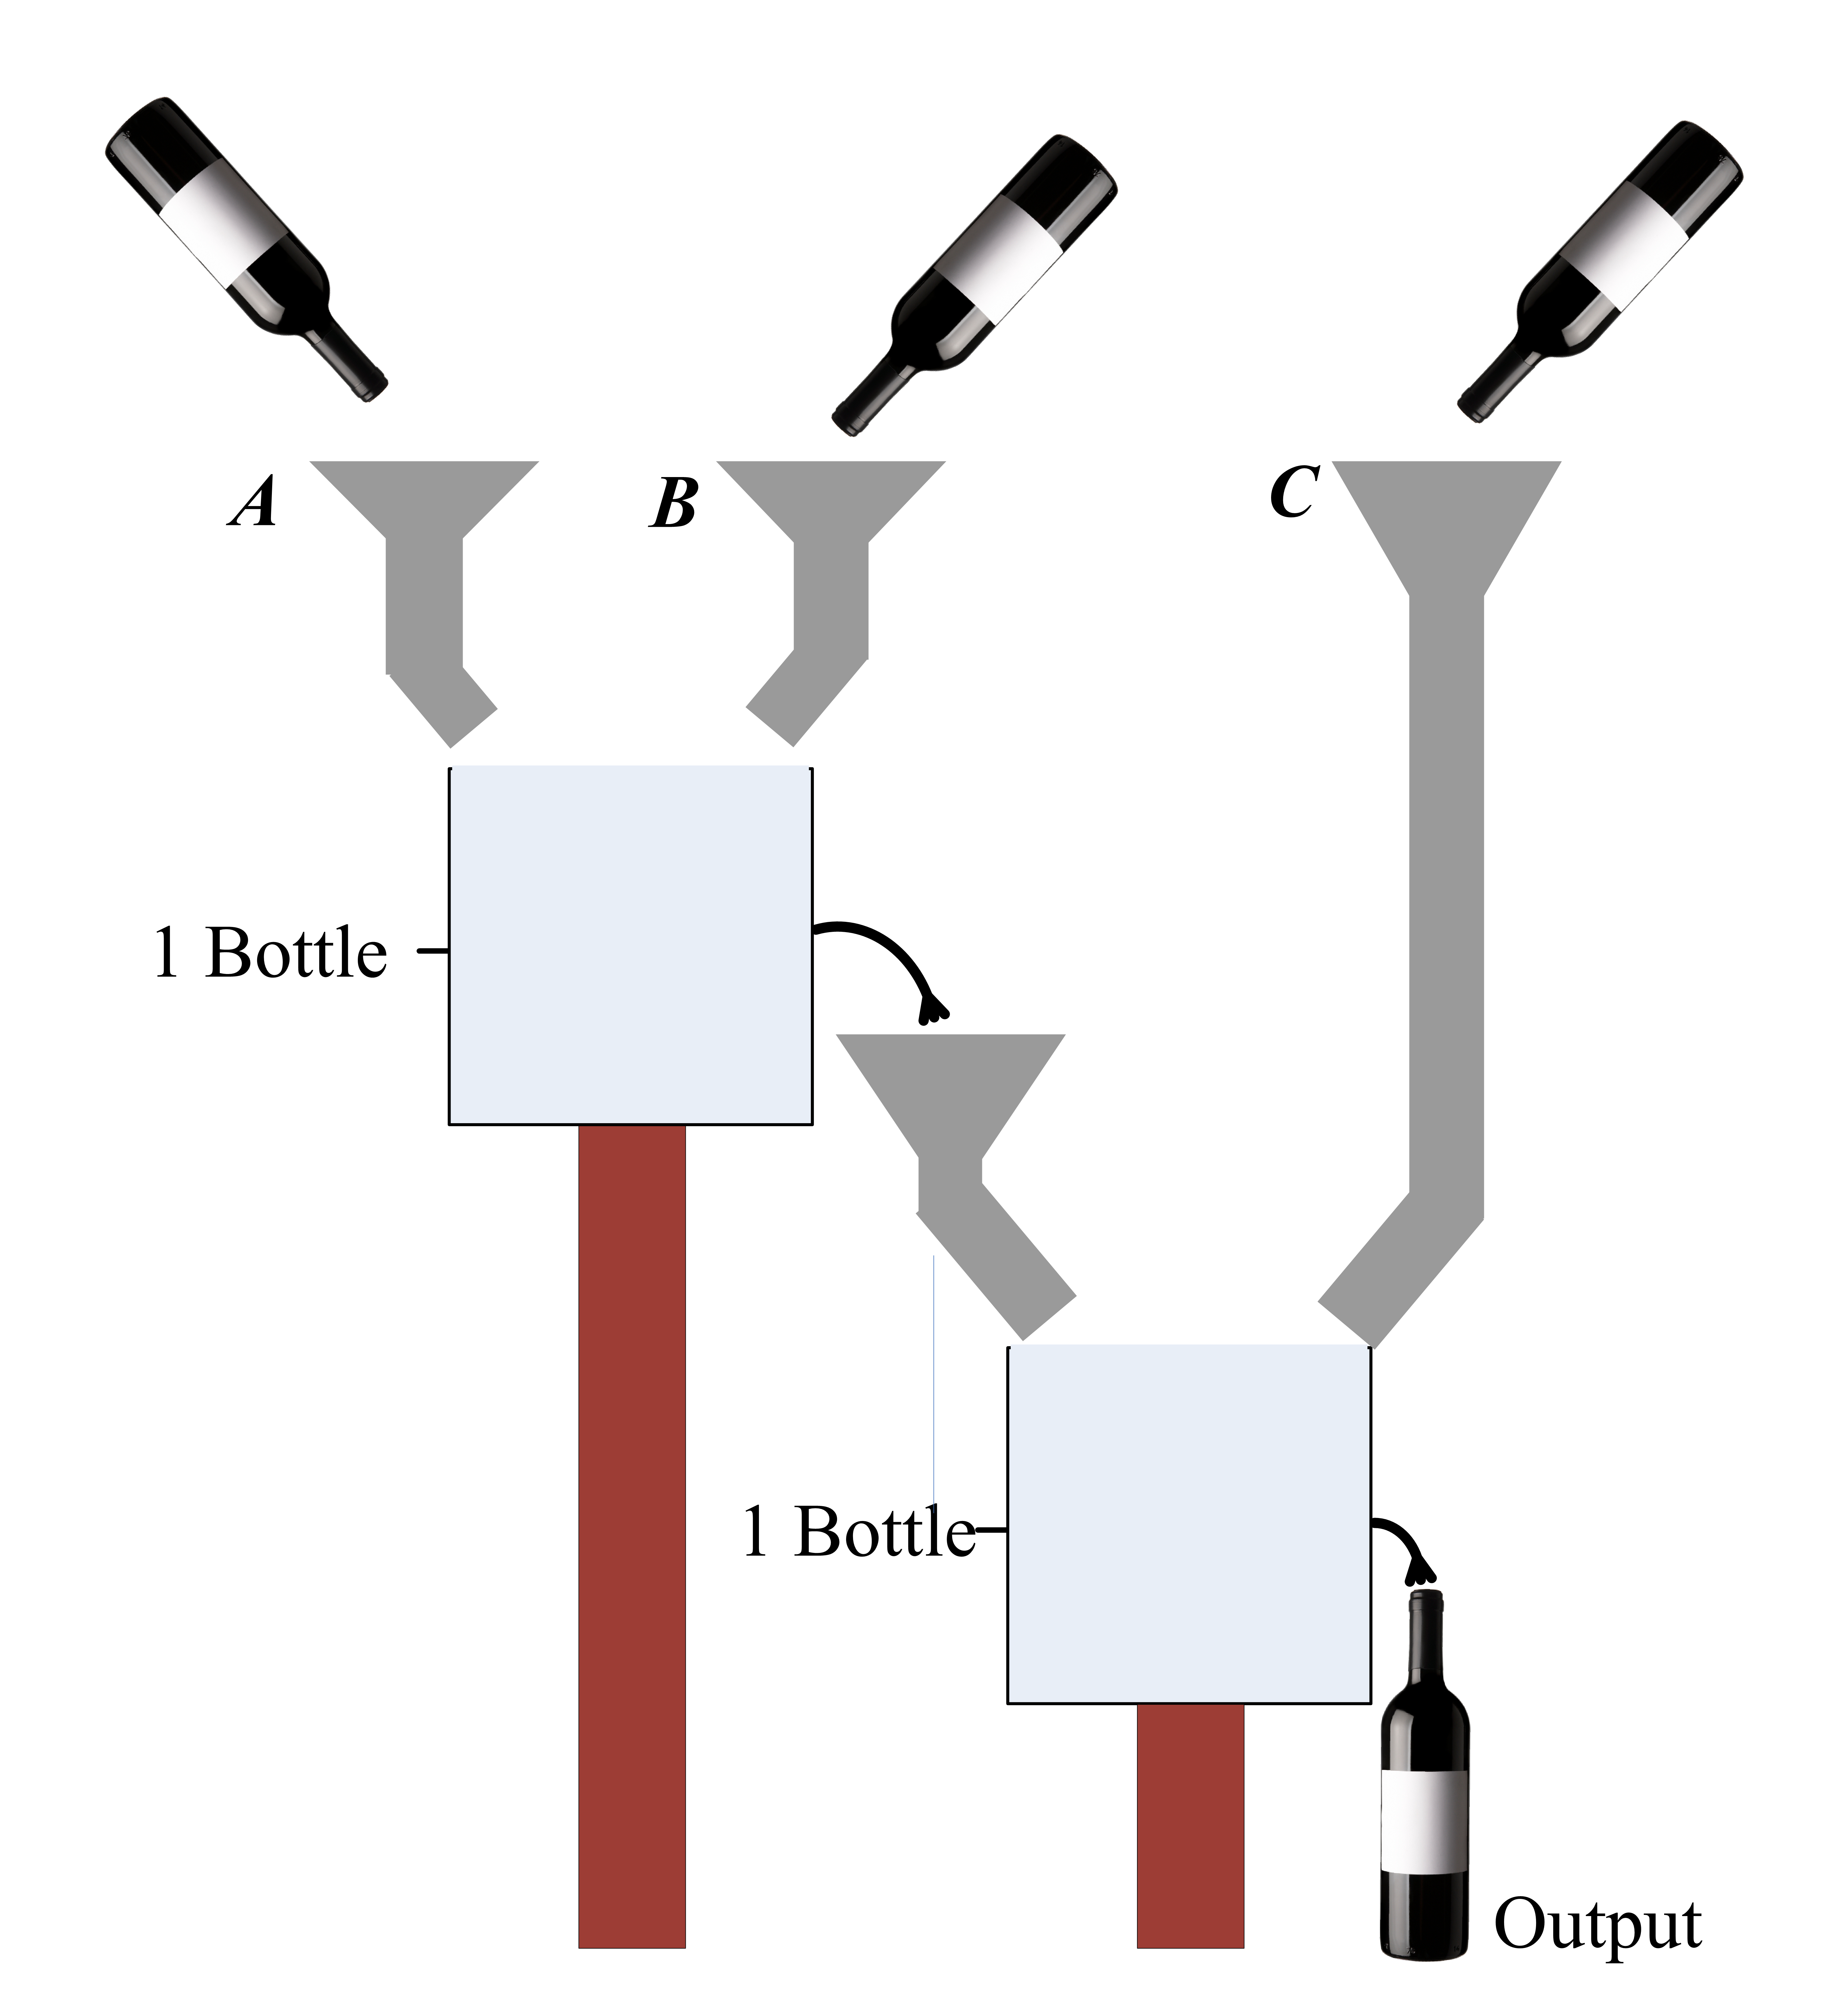
\includegraphics{figures/three-and.png}}} 
\end{center}
\caption{Computing \function{and3} by composing two \function{and} functions.\label{fig:three-and-compose}}
\end{figure}

Composing logical functions also allows us to build new logical functions.  Consider the \function{xor} (exclusive or) function that takes two inputs, and has output \true\ when exactly one of the inputs is \true:  
\begin{center}
	\begin{tabular}{cc|c} %\hline
		%\multicolumn{2}{|c|}{\bf Inputs} & {\bf Output} \\ 
		\var{A} & \var{B} & \scheme|(xor A B)|\\ \hline
		\false & \false & \false \\
		\true & \false & \true \\
		\false & \true & \true \\
		\true & \true & \false \\ 
	\end{tabular}
\end{center}


\LATER{
The \function{xor} function has the useful property that performing it twice always produces the original value: \scheme|(xor (xor A B) B)| $\equiv$ \var{A} for any Boolean values \var{A} and \var{B}\LATER{(in Exploration~\ref{excur:colossus}, we see why this property is very useful for cryptography)}. Here, we are xor-ing \var{A} with \var{B} in the inner \function{xor}; then, the result is xor-ed with \var{B} again.  No matter what \var{B} is the result is the value of \var{A}.  There are several ways to see this.  Since there are only two possible choices for \var{A}, and two possible choices for \var{B}, we can try all four possibilities and show the equation holds (see Exercise~\ref{exercise:xor} for another way to show this).}

Can we build \function{xor} by composing the functions we already have?  

The \function{xor} is similar to \function{or}, except for the result when both inputs are \true.  So, we could compute \scheme|(xor A B)| as
\scheme|(and (or A B) (not (and A B)))|.  Thus, we can build an \function{xor} machine by composing the designs we already have for \function{and}, \function{or}, and \function{not}. 

\cut{
Another approach is to observe that \scheme|(xor A B)| is \true\ in only two situations: (1) when \var{A} is \true\ and \var{B} is \false, and (2) when \var{A} is \false\ and \var{B} is \true.  Hence, we can compute \scheme|(xor A B)| by using the \function{or} function to combine these two situations: \scheme|(or (and A (not B)) (and (not A) B))|.  The first input to the \function{or} function is \true\ only if the first situation holds, and the second input is \true\ only if the second situation holds, so the \function{or} will be \true\ only if at least one of the clauses is \true.}  

We can compose any pair of functions where the outputs for the first function are consistent with the input for the second function.  One particularly important function known as \function{nand} results from \function{not} and \function{and}:

\begin{center}
	\begin{tabular}{cc|c} %\hline
		%\multicolumn{2}{|c|}{\bf Inputs} & {\bf Output} \\ 
		\var{A} & \var{B} & (\function{nand} \var{A} \var{B}) \\ \hline
		\false & \false & \true \\
		\true & \false & \true \\
		\false & \true & \true \\
		\true & \true & \false \\ % \hline	
	\end{tabular}
\end{center}

\emph{All} Boolean logic functions can be implemented using just the \function{nand} function.  One way to prove this is to show how to build all logic functions using just \function{nand}.  For example, we can implement \function{not} using \function{nand} where the one input to the \function{not} function is used for both inputs to the \function{nand} function: 
\begin{center}
\scheme|(not A)| $\equiv$ \scheme|(nand A A)|
\end{center}
Now that we have shown how to implement \function{not} using \function{nand}, it is easy to see how to implement \function{and} using \function{nand}:
\begin{center}
\scheme|(and A B)| $\equiv$ \scheme|(not (nand A B))|
\end{center}

Implementing \function{or} is a bit trickier.  Recall that \var{A} \function{or} \var{B} is \true\ if any one of the inputs is \true.  But, \var{A} \function{nand} \var{B} is \true\ if both inputs are \false, and \false\ if both inputs are \true.  To compute \function{or} using only \function{nand} functions, we need to invert both inputs:
\begin{center}
\scheme|(or A B)| $\equiv$ \scheme|(nand (not A) (not B))|
\end{center}

To complete the proof, we would need to show how to implement all the other Boolean logic functions.  We omit the details here, but leave some of the other functions as exercises.  The universality of the \function{nand} function makes it very useful for implementing computing devices.  Trillions of \function{nand} gates are produced in silicon every day.

\beforeex
\begin{exercise}
Define a Scheme procedure, \scheme|logical-or|, that takes two inputs and outputs the logical or of those inputs.
\solution{
\begin{schemedisplay}
(define (logical-or a b) (if a true b))
\end{schemedisplay}
}
\end{exercise}
\afterex

\beforeex
\begin{exercise}\label{ex:notnot}
What is the meaning of composing \function{not} with itself?  For example, (\function{not} (\function{not} \var{A})).
\solution{
It is an identity function: for any \var{A}, (\function{not}(\function{not} \var{A})) = \var{A}.
}
\end{exercise}
\afterex

\beforeex
\begin{exercise}
\bluestar Define the \function{xor} function using only \function{nand} functions.
\solution{
(\function{xor} \var{A} \var{B}) $\equiv$ (\function{and} (\function{or} \var{A} \var{B}) (\function{nand} \var{A} \var{B})).  The book already describes how to express \function{and}, \function{not}, and \function{or} in terms of\function{nand}, so we can plug in those definition to obtain a full definition of \function{xor} using only \function{nand}.
}
\end{exercise}
\afterex

% exercises: how well does this work? inputs are .6 and .6, output is <1.2?

\LATER{
\ex{\greenstar \label{exercise:xor}
Another way to see that \scheme|(xor (xor A B) B)| $\equiv$ \var{A} is to first argue that \function{xor} operations are {\em commutative}.  This means we can change the order in which they are performed without changing the result.  That is, 
\begin{center}
(\function{xor} (\function{xor} \var{A} \var{B}) \var{C}) $\equiv$ (\function{xor} \var{A} (\function{xor} \var{B} \var{C}))
\end{center}
Prove that \function{xor} is commutative, and use this result to show that the inversion property holds. 
}}

\beforeex
\begin{exercise} \goldstar \label{ex:copy}
Our definition of \scheme|(not A)| as \scheme|(nand A A)| assumes there is a way to produce two copies of a given input.  Design a component for our wine machine that can do this.  It should take one input, and produce two outputs, both with the same value as the input.  (Hint: when the input is \true, we need to produce two full bottles as outputs, so there must be a source similarly to the \function{not} component.)
\solution{
It is very similar to the \function{not} machine. The difference is that the two nozzles are at the bottom
of the basin (below the float) and fill two bottles of wine. The source's outlet is also at the
bottom blocked by the float when the input is empty. If the input is a full bottle, then the
float would unblock the source and fill the two bottles.
}
\end{exercise}
\afterex

\beforesplitex
\begin{exercise} \goldstar \label{ex:amplifier}
The digital abstraction works fine as long as actual values stay close to the value they represent.  But, if we continue to compute with the outputs of functions, the actual values will get increasingly fuzzy.  For example, if the inputs to the \function{and3} function in Figure~\ref{fig:three-and-compose} are initially all $\frac{3}{4}$ full bottles (which should be interpreted as \true), the basin for the first \function{and} function will fill to $1\frac{1}{2}$, so only $\frac{1}{2}$ bottle will be output from the first \function{and}.  When combined with the third input, the second basin will contain $1\frac{1}{4}$ bottles, so only $\frac{1}{4}$ will spill into the output bottle.  Thus, the output will represent \false, even though all three inputs represent \true.  The solution to this problem is to use an \emph{amplifier} to restore values to their full representations.  Design a wine machine amplifier that takes one input and produces a strong representation of that input as its output.  If that input represents \true\ (any value that is half full or more), the amplifier should output \true, but with a strong, full bottle representation.  If that input represents \false\ (any value that is less than half full), the amplifier should output a strong \false\ value (completely empty).  
\solution{
This is a use case for the identify function from
Exercise~\ref{ex:notnot}: two \function{not} machines should be combined to
produce the desired amplifier.

}
\end{exercise}
\aftersplitex

\LATER{
\excur{Colossus\label{excur:colossus}}{
\TODO{The \function{xor}}}
}

\subsection{Arithmetic}\label{sec:binaryarithmetic}

Not only is the \function{nand} function complete for Boolean logical functions, it is also enough to implement all discrete arithmetic functions.  
%We show how to compute addition using only \function{nand} functions.  
First, consider the problem of adding two one-bit numbers.  

\groupcontent{
There are four possible pairs of inputs:
\begin{center}
	\begin{tabular}{cccccc} 
		%\multicolumn{3}{c}{\bf Inputs} & & \multicolumn{2}{c}{\bf Output} \\ 
		\var{A} & & \var{B} & & $r_1$ & $r_0$ \\ \hline
		\bO & + & \bO & = & \bO & \bO \\
		\bO & + & \bI & = & \bO & \bI \\
		\bI & + & \bO & = & \bO & \bI \\
		\bI & + & \bI & = & \bI & \bO \\ 
	\end{tabular}
\end{center}
}

We can compute each of the two output bits as a logical function of the two input bits.  The right output bit, $r_0$, is \bI\ if exactly one of the input bits is \bI:
\begin{center}
$r_0$ = \scheme|(or (and (not A) B) (and A (not B)))|
\end{center}
This is what the \function{xor} function computes, so:
\begin{center}
$r_0$ = \scheme|(xor A B)|
\end{center}

The left output bit, $r_1$, is \bO\ for all inputs except when both inputs are \bI:
\begin{center}
$r_1$ = \scheme|(and A B)|
\end{center}
Since we have already seen how to implement \function{and}, \function{or}, \function{xor}, and \function{not} using only \function{nand} functions, this means we can implement a one-bit adder using only \function{nand} functions.

Adding larger numbers requires more logical functions.  Consider adding two $n$-bit numbers:
\begin{tabbing} 
\hspace*{2cm}  \= \qquad \= \qquad \= \quad\qquad\= \quad\qquad \= \quad\qquad\= \qquad\=  \kill
               \>       \>       \> $a_{n-1}$  \> $a_{n - 2}$ \> $\cdots$   \> $a_1$ \> $a_0$ \\
               \>  +    \>       \> $b_{n-1}$ \> $b_{n - 2}$ \> $\cdots$ \> $b_1$ \> $b_0$ \\[-0.5ex]
               \>    \> \rule{5.5cm}{0.2mm} \\[0ex]
               \>  =  \> $r_{n}$ \> $r_{n-1}$ \> $r_{n - 2}$ \> $\cdots$ \> $r_1$ \> $r_0$ \\
\end{tabbing}

The elementary school algorithm for adding decimal numbers is to sum up the digits from right to left.  If the result in one place is more than one digit, the additional tens are carried to the next digit.  We use $c_k$ to represent the carry digit in the $k^{th}$ column.

\groupcontent{
\begin{tabbing} 
\hspace*{2cm}  \= \qquad \= \qquad    \= \quad\qquad\= \quad\qquad \= \quad\qquad\= \qquad \=  \kill
               \>       \> $c_{n}$  \> $c_{n-1}$  \> $c_{n - 2}$ \> $\cdots$   \> $c_1$  \> \\
               \>       \>          \> $a_{n-1}$  \> $a_{n - 2}$ \> $\cdots$   \> $a_1$  \> $a_0$ \\
               \>  +    \>          \> $b_{n-1}$  \> $b_{n - 2}$ \> $\cdots$   \> $b_1$  \> $b_0$ \\[-0.5ex]
               \>       \> \rule{5.5cm}{0.2mm} \\[0ex]
               \>  =    \> $r_{n}$ \> $r_{n-1}$   \> $r_{n - 2}$ \> $\cdots$ \> $r_1$ \> $r_0$ \\
\end{tabbing}
}

The algorithm for addition is:
\begin{itemtight}
\item Initially, $c_{0} = 0$.
\item Repeat for each digit $k$ from $0$ to $n$: 
\begin{enumtight}\vspace*{1.5ex}
\item $v_1v_0 = a_k + b_k + c_k$ (if there is no digit $a_k$ or $b_k$ use $0$).
\item $r_k$ = $v_0$.
\item $c_{k+1} = v_1$.
\end{enumtight}
\end{itemtight}

This is perhaps the first interesting algorithm most people learn: if followed correctly, it is guaranteed to produce the correct result, and to always finish, for any two input numbers.

Step 1 seems to require already knowing how to perform addition, since it uses $+$.  But, the numbers added are one-digit numbers (and $c_k$ is $0$ or $1$).  Hence, there are a finite number of possible inputs for the addition in step 1: 10 decimal digits for $a_k$ $\times$ 10 decimal digits for $b_k$ $\times$ 2 possible values of $c_k$.  We can memorize the 100 possibilities for adding two digits (or write them down in a table), and easily add one as necessary for the carry.  Hence, computing this addition does not require a general addition algorithm, just a specialized method for adding one-digit numbers.

We can use the same algorithm to sum binary numbers, except it is simpler since there are only two binary digits.  Without the carry bit, the result bit, $r_k$, is \bI\ if \scheme|(xor \ak \bk)|.  If the carry bit is \bI, the result bit should flip.  So,
\begin{centernospace}
$r_k$ = \scheme|(xor (xor \ak \bk) \ck)|
\end{centernospace}
This is the same as adding $a_k + b_k + c_k$ base two and keeping only the right digit.

The carry bit is \bI\ if the sum of the input bits and previous carry bit is greater than \schemeresult|1|.  This happens when any two of the bits are \bI:
\begin{centernospace}
$c_{k+1}$ = \scheme|(or (and \ak \bk) (and \ak \ck) (and \bk \ck))|
\end{centernospace}

As with elementary school decimal addition, we start with $c_{0} = 0$, and proceed through all the bits from right to left.

We can propagate the equations through the steps to find a logical equation for each result bit in terms of just the input bits.  First, we simplify the functions for the first result and carry bits based on knowing $c_0 = 0$:
\begin{tabbing}
\hspace{.2in} \= $r_0$ \= = \scheme|(xor (xor \az \bz) \cz)| = \scheme|(xor \az \bz)| \\
              \> $c_1$ \> = \scheme|(or (and \az \bz) (and \az \cz) (and \bz \cz))| = \scheme|(and \az \bz)|
\end{tabbing}
Then, we can derive the functions for $r_1$ and $c_2$:
\begin{tabbing}
\hspace{.2in} \= $r_1$ \= = \scheme|(xor (xor \aone \bone) \cone)| = \scheme|(xor (xor \aone \bone) (and \az \bz))|\\
              \> $c_2$ \> = \scheme|(or (and \aone \bone) (and \aone \cone) (and \bone \cone))| \\
              \>       \> = \scheme|(or (and \aone \bone) (and \aone (and \az \bz)) (and \bone (and \az \bz)))|
\end{tabbing}

As we move left through the digits, the terms get increasingly complex.  But, for any number of digits, we can always find functions for computing the result bits using only logical functions on the input bits.  Hence, we can implement addition for any length binary numbers using only \function{nand} functions.

%For example, $r_3$ is:
%\begin{schemedisplay}
%(xor (xor \athree \bthree) 
%     (or (and \atwo \btwo) 
%         (and \atwo (or (and \aone \bone) 
%                        (and \aone (and \az \bz)) 
%                        (and \bone (and \az \bz)))) 
%         (and \btwo (or (and \aone \bone) 
%                        (and \aone (and \az \bz)) 
%                        (and \bone (and \az \bz))))))
%\end{schemedisplay}
%r_2 = (xor (xor \a2 \b2) (or (and \aone \bone) (and \aone (and \ak \bk)) (and \bone (and \ak \bk))))
%c_3 = (or (and \a2 \b2) (and \a2 (or (and \aone \bone) (and \aone (and \az \bz)) (and \bone (and \az \bz)))) (and \b2 (or (and \aone \bone) (and \aone (and \az \bz)) (and \bone (and \az \bz)))))
%r_3 = (xor (xor \a3 \b3) (or (and \a2 \b2) (and \a2 (or (and \aone \bone) (and \aone (and \az \bz)) (and \bone (and \az \bz)))) (and \b2 (or (and \aone \bone) (and \aone (and \az \bz)) (and \bone (and \az \bz))))))

We can also implement multiplication, subtraction, and division using only \function{nand} functions.  We omit the details here, but the essential approach of breaking down our elementary school arithmetic algorithms into functions for computing each output bit works for all of the arithmetic operations.

\beforeex
\begin{exercise}
Adding logically.
\begin{subexerciselist}
\item What is the logical formula for $r_3$?
\solution{
\begin{schemedisplay}
r2 = (xor (xor a2 b2) c2) 
   = (xor (xor a2 b2)
          (or (and a1 b1) (and a1 (and a0 b0)) (and b1 (and a0 b0))))

c3 = (or (and a2 b2) (and a2 c2) (and b2 c2))
   = (or (and a2 b2)
         (and a2 (or (and a1 b1) (and a1 (and a0 b0)) (and b1 (and a0 b0))))
         (and b2 (or (and a1 b1) (and a1 (and a0 b0)) (and b1 (and a0 b0)))))

r3 = (xor (xor a3 b3) c3)
   = (xor (xor a3 b3)
          (or (and a2 b2)
              (and a2 (or (and a1 b1) (and a1 (and a0 b0)) (and b1 (and a0 b0))))
              (and b2 (or (and a1 b1) (and a1 (and a0 b0)) (and b1 (and a0 b0))))))

c4= (or (and a3 b3) (and a3 c3) (and b3 c3))

r4 = (xor (xor a4 b4) c4)
\end{schemedisplay}
}
\item Without simplification, how many functions will be composed to compute the addition result bit $r_4$?  
\solution{
The number of functions (without simplification) for $c_k$ is $4+2c_{k-1}$ for $k>1$, and $c_1 = 1$. Thus, $c_2 = 6$, $c_3 = 16$, and $c_4=36$. 

The number of functions (without simplification) for $r_k$ is $2+c_k$ for $k > 0$. Thus, $r_1 = 3$, $r_2 = 8$, $r_3=18$, and $r_4 = 38$.

}
\item \goldstar Is it possible to compute $r_4$ with fewer logical functions?
\solution{
Yes --- we can considerably simplify the expression of $r_4$ by observing that we can get:
\begin{schemedisplay}
c2 = (or (and a1 b1) (and c1 (or a1 b1))) 
   = (or (and a1 b1) (and (and a0 b0) (or a1 b1)))
\end{schemedisplay}
Or more generally:
\begin{schemedisplay}
ck = (or (and ak bk) (and c[k-1] (or ak bk)))
\end{schemedisplay}

We may simplify both $c_3$ and $c_4$ via the previous template. We'll
leave proving the minimal number of operations as a \doublegoldstar exercise.
}
\end{subexerciselist}
\end{exercise}
\afterex

\beforeex
\begin{exercise} \bluestar 
Show how to compute the result bits for binary multiplication of two 2-bit inputs using only logical functions.
\solution{
The multiplication of two 2-bits numbers is comprised from one-bit multiplications and
additions. Suppose we multiply $a_1a_0$ with $b_1b_0$. We get the following result bits (the carry
bits are presented for better clarity):
\begin{schemedisplay}
r0 = (and a0 b0)
c0 = 0

r1 = (xor (and a0 b1) (and a1 b0))
c1 = (and (and a0 b1) (and a1 b0))

r2 = (xor (and a1 b1) c1) = (xor (and a1 b1) (and (and a0 b1) (and a1 b0)))
c2 = (and (and a1 b1) c1) = (and (and a1 b1) (and (and a0 b1) (and a1 b0)))

r3 = c2 = (and (and a1 b1) c1) = (and (and a1 b1) (and (and a0 b1) (and a1 b0)))
\end{schemedisplay}
}
\end{exercise}
\afterex

\beforeex
\begin{exercise} \goldstar 
Show how to compute the result bits for binary multiplication of two inputs of any length using only logical functions.
\solution{

The number of logical functions needed is quite large even for a tiny
example of multiplying 2-bit by 2-bit numbers. In a general case, we
cannot use such na\"{i}ve approach.  A classical two $n$-bit
multiplier applies a shifter and accumulator to sum up partial
products (this is known as shift-and-add multiplication). Modern
architectures are much faster and employ quite advanced algorithms and
hardware. You may want to look up Wallace Trees and Dadda Multipliers
to get some ideas how to do this.

}

\end{exercise}
\afterex

\section{Modeling Computing}\label{sec:modeling}

By composing the logic functions, we could build a wine computer to perform any Boolean function.  And, we can perform any discrete arithmetic function using only Boolean functions.  For a useful computer, though, we need programmability.  We would like to be able to make the inputs to the machine describe the logical functions that it should perform, rather than having to build a new machine for each desired function.  We could, in theory, construct such a machine using wine, but it would be awfully complicated.  Instead, we consider programmable computing machines abstractly. 

Recall in Chapter~\ref{ch:intro}, we defined a computer as a machine that can:
\begin{enumtight}
\item Accept input.  
\item Execute a mechanical procedure. 
\item Produce output.
\end{enumtight}
So, our model of a computer needs to model these three things.  

\shortsection{Modeling input} In real computers, input comes in many forms: typing on a keyboard, moving a mouse, packets coming in from the network, an accelerometer in the device, etc.  

%\begin{figure}[!bth]
%\begin{center}
%{\scalebox{0.65}{\includegraphics{images/input-devices.png}}}
% images from istockPhoto
%\caption{Sample input devices.}
%\subcapc{Keyboard, mouse, camera, touchscreen, and microphone.}
%\end{center}
%\end{figure}

\sidepicturenocap{1.0}{images/mouse-iStock_000002492027XSmall.jpg}
For our model, we want to keep things as simple as possible, though.  From a computational standpoint, it doesn't really matter how the input is collected.  We can represent any discrete input with a sequence of bits.  Input devices like keyboards are clearly discrete: there are a finite number of keys, and each key could be assigned a unique number.  Input from a pointing device like a mouse could be continuous, but we can always identify some minimum detected movement distance, and record the mouse movements as discrete numbers of move units and directions.  Richer input devices like a camera or microphone can also produce discrete output by discretizing the input using a process similar to the image storage in Chapter~\ref{ch:intro}.  So, the information produced by any input device can be represented by a sequence of bits.  

\sidequote{The virtual shopping spree was a first for the President who has a reputation for being ``technologically challenged.'' But White House sources insist that the First Shopper used his own laptop and even ``knew how to use the mouse.''}{BusinessWeek, 22~December~1999}
For real input devices, the time an event occurs is often crucial.  When playing a video game, it does not just matter that the mouse button was clicked, it matters a great deal \emph{when} the click occurs.  How can we model inputs where time matters using just our simple sequence of bits?  

One way would be to divide time into discrete quanta \cut{(as discussed in the footnote on page~\pageref{footnote:time}, it is not known if time is actually discrete or continuous, but we can sensibly divide time into small enough quanta that the quantization is imperceptible to a human)}and encode the input as zero or one events in each quanta.  A more efficient way would be to add a timestamp to each input.  The timestamps are just numbers (e.g., the number of milliseconds since the start time), so can be written down just as sequences of bits.

Thus, we can model a wide range of complex input devices with just a finite sequence of bits.  The input must be finite, since our model computer needs all the input before it starts processing.  This means our model is not a good model for computations where the input is infinite, such as a web server intended to keep running and processing new inputs (e.g., requests for a web page) forever.  In practice, though, this isn't usually a big problem since we can make the input finite by limiting the time the server is running in the model.

A finite sequence of bits can be modeled using a long, narrow, tape that is divided into squares, where each square contains one bit of the input.
\sidepicturenocap{0.2}{images/touchscreen-iStock_000000892290XSmall.jpg}

\shortsection{Modeling output} Output from computers effects the physical world in lots of very complex ways: displaying images on a screen, printing text on a printer, sending an encoded web page over a network, sending an electrical signal to an anti-lock brake to increase the braking pressure, etc.  

%\begin{figure}[!bth]
%\begin{center}
%{\scalebox{0.65}{\includegraphics{images/output-devices.png}}}
% images from istockPhoto
%\caption{Sample output devices.}
%\subcapc{Monitor, multi-screen display, printer, and speakers.}
%\end{center} 
%\end{figure}

We don't attempt to model the physical impact of computer outputs; that would be far too complicated, but it is also one step beyond modeling the computation itself.  Instead, we consider just the information content of the output.  The information in a picture is the same whether it is presented as a sequence of bits or an image projected on a screen, its just less pleasant to look at as a sequence of bits.  So, we can model the output just like we modeled the input: a sequence of bits written on a tape divided into squares.

\shortsection{Modeling processing}  Our processing model should be able to model every possible mechanical procedure since we want to model a universal computer, but should be as simple as possible.  

One thing our model computer needs is a way to keep track of what it is doing.  We can think of this like scratch paper: a human would not be able to do a long computation without keeping track of intermediate values on scratch paper, and a computer has the same need.  In Babbage's Analytical Engine, this was called the \emph{store}, and divided into a thousand variables, each of which could store a fifty decimal digit number.  In the Apollo Guidance Computer, the working memory was divided into banks, each bank holding 1024 words.  Each word was 15 bits (plus one bit for error correction).  In current 32-bit processors, such as the x86, memory is divided into pages, each containing 1024 32-bit words.  

For our model machine, we don't want to have arbitrary limits on the amount of working storage.  So, we model the working storage with an infinitely long tape.  Like the input and output tapes, it is divided into squares, and each square can contain one symbol.  For our model computer, it is useful to think about having an infinitely long tape, but of course, no real computer has infinite amounts of working storage.  We can, however, imagine continuing to add more memory to a real computer as needed until we have enough to solve a given problem, and adding more if we need to solve a larger problem.  

Our model now involves separate tapes for input, output, and a working tape.  We can simplify the model by using a single tape for all three.  At the beginning of the execution, the tape contains the input (which must be finite).  As processing is done, the input is read and the tape is used as the working tape.  Whatever is on the tape and the end of the execution is the output.\LATER{adding tapes doesn't make our model machine more powerful}

We also need a way for our model machine to interface with the tape.  We imagine a tape head that contacts a single square on the tape.  On each processing step, the tape head can read the symbol in the current square, write a symbol in the current square, and move one square either left or right.  

The final thing we need is a way to model actually doing the processing.  In our model, this means controlling what the tape head does: at each step, it needs to decide what to write on the tape, and whether to move left or right, or to finish the execution.  %Babbage called the processor the \emph{mill}; in modern computers, it is called the \emph{central processing unit} (CPU).

In early computing machines, processing meant performing one of the basic arithmetic operations (addition, subtraction, multiplication, or division).  We don't want to have to model anything as complex as multiplication in our model machine, however.  The previous section showed how addition and other arithmetic operations can be built from simpler logical operations.  To carry out a complex operation as a composition of simple operations, we need a way to keep track of enough state to know what to do next. The machine state is just a number that keeps track of what the machine is doing.  Unlike the tape, it is limited to a finite number.  There are two reasons why the machine state number must be finite: first, we need to be able to write down the program for the machine by explaining what it should do in each state, which would be difficult if there were infinitely many states.

We also need rules to control what the tape head does.  We can think of each rule as a mapping from the current observed state of the machine to what to do next.  The input for a rule is the symbol in the current tape square and the current state of the machine; the output of each rule is three things: the symbol to write on the current tape square, the direction for the tape head to move (left, right, or halt), and the new machine state.  We can describe the program for the machine by listing the rules.  For each machine state, we need a rule for each possible symbol on the tape.

%https://www.cs.tcd.ie/Glenn.Strong/3d5/project1.pdf

\subsection{Turing Machines}\index{general}{Turing Machine}\index{people}{Turing, Alan}

This abstract model of a computer was invented by Alan Turing in the 1930s and is known as a \emph{Turing Machine}.  
Turing's model is depicted in Figure~\ref{fig:tm}.  An infinite tape divided into squares is used as the input, working storage, and output.  The tape head can read the current square on the tape, write a symbol into the current tape square, and move left or right one position.  The tape head keeps track of its internal state, and follows rules matching the current state and current tape square to determine what to do next.  

Turing's model is by far the most widely used model for computers today.  Turing developed this model in 1936, before anything resembling a modern computer existed.  Turing did not develop his model as a model of an automatic computer, but instead as a model for what could be done by a human following mechanical rules.  He devised the infinite tape to model the two-dimensional graph paper students use to perform arithmetic.  He argued that the number of machine states must be limited by arguing that a human could only keep a limited amount of information in mind at one time.  

\begin{figure}[bt]
\begin{center}
\vspace*{1.0ex}
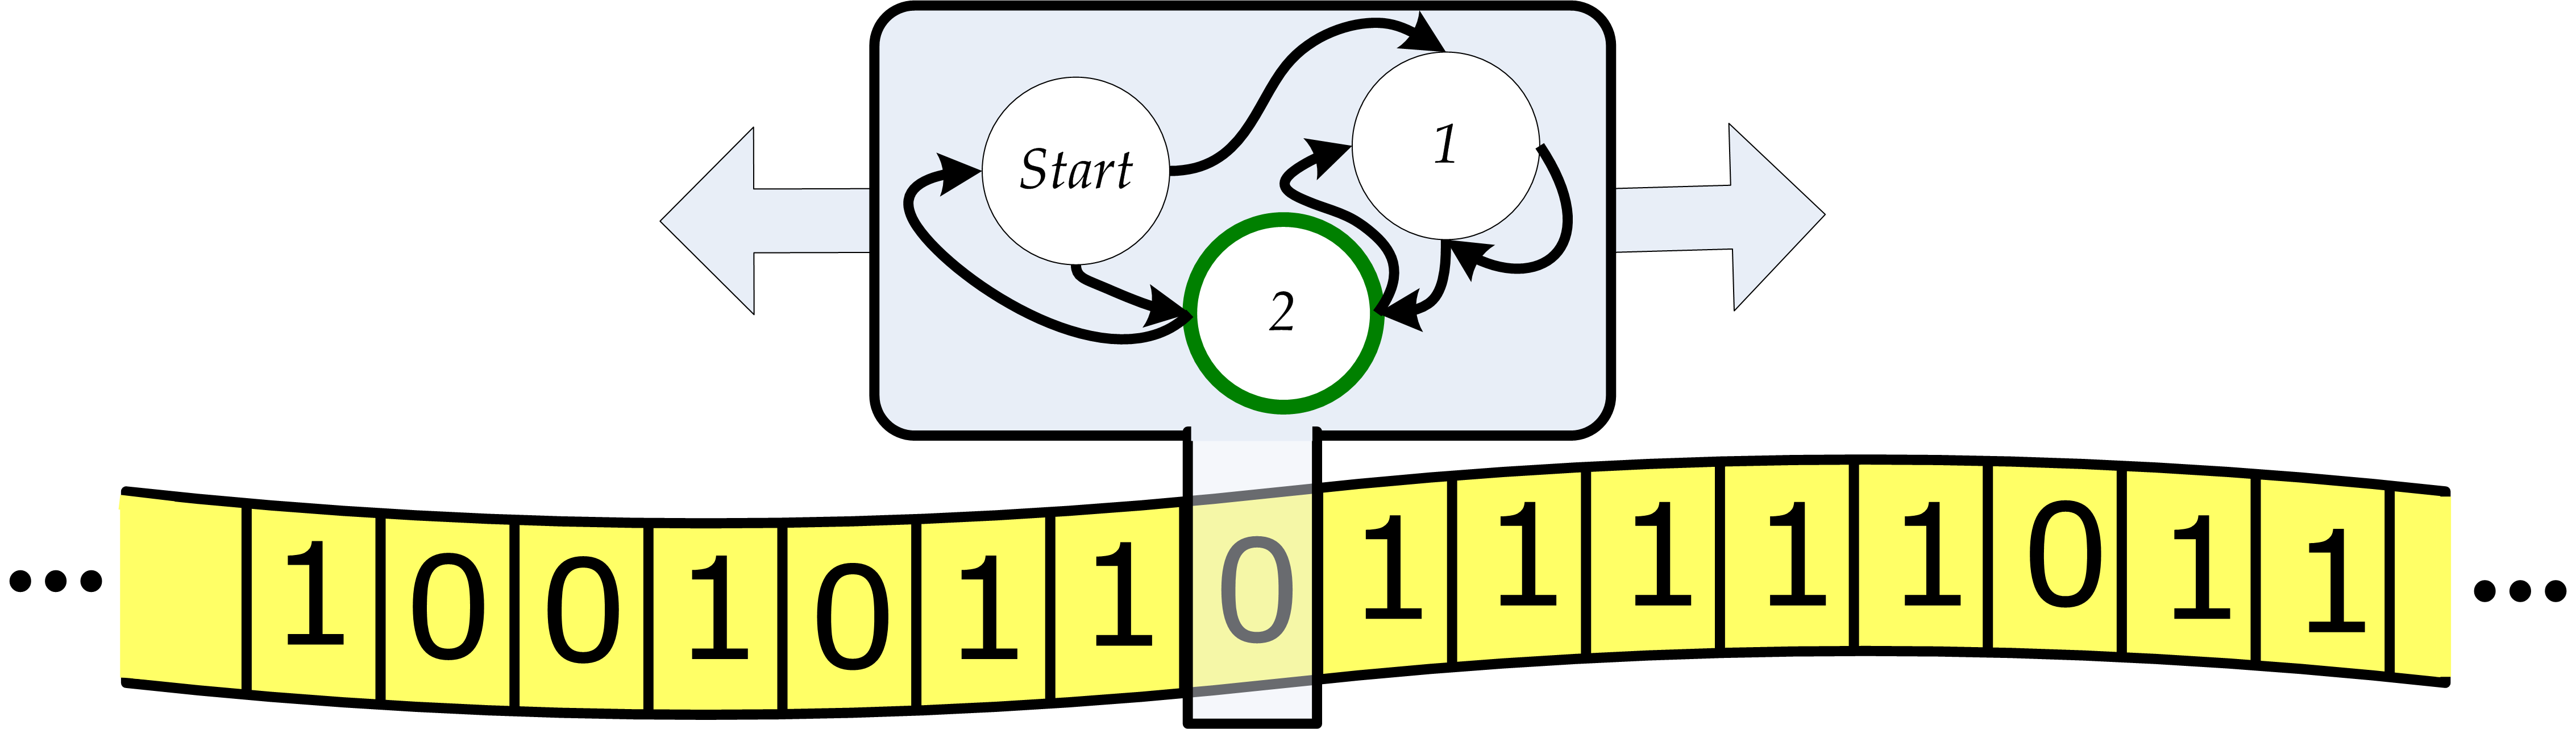
\includegraphics[width=4.8in]{figures/tm-model.png}
\caption{Turing Machine model.\label{fig:tm}}
\end{center} 
\end{figure}

Turing's model is equivalent to the model we described earlier, but instead of using only bits as the symbols on the tape, Turing's model uses members of any finite set of symbols, known as the \emph{alphabet} of the tape.  Allowing the tape alphabet to contain any set of symbols instead of just the two binary digits makes it easier to describe a Turing Machine that computes a particular function, but does not change the power of the model.  That means, every computation that could be done with a Turing Machine using any alphabet set, could also be done by some Turing Machine using only the binary digits.  

We could show this by describing an algorithm that takes in a description of a Turing Machine using an arbitrarily large alphabet, and produces a Turing Machine that uses only two symbols to simulate the input Turing Machine.  As we saw in Chapter~\ref{ch:intro}, we can map each of the alphabet symbols to a finite sequence of binary digits.  

Mapping the rules is more complex: since each original input symbol is now spread over several squares, we need extra states and rules to read the equivalent of one original input.  For example, suppose our original machine uses 16 alphabet symbols, and we map each symbol to a 4-bit sequence.  If the original machine used a symbol \verb+X+, which we map to the sequence of bits \verb+1011+, we would need four states for every state in the original machine that has a rule using \verb+X+ as input.  These four states would read the \verb+1+, \verb+0+, \verb+1+, \verb+1+ from the tape.  The last state now corresponds to the state in the original machine when an \verb+X+ is read from the tape.  To follow the rule, we also need to use four states to write the bit sequence corresponding to the original write symbol on the tape.  Then, simulating moving one square left or right on the original Turing Machine, now requires moving four squares, so requires four more states.  Hence, we may need 12 states for each transition rule of the original machine, but can simulate everything it does using only two symbols.

The Turing Machine model is a \definition{universal computing machine}.  This means every algorithm can be implemented by some Turing Machine.  \cut{We call a system that can implement every algorithm \emph{Turing complete}.  A system that is Turing complete can simulate every possible Turing Machine.}  Chapter~\ref{ch:universal} explores more deeply what it means to simulate every possible Turing Machine and explores the set of problems that can be solved by a Turing Machine.  

Any physical machine has a limited amount of memory.  If the machine does not have enough space to store a trillion bits, there is no way it can do a computation whose output would exceed a trillion bits.  Nevertheless, the simplicity and robustness of the Turing Machine model make it a useful way to think about computing even if we cannot build a truly universal computing machine.

Turing's model has proven to be remarkably robust.  Despite being invented before anything resembling a modern computer existed, nearly every computing machine ever imagined or built can be modeled well using Turing's simple model.\cut{\footnote{In Chapter~\ref{ch:alternatemodels}, we describe a few machines that cannot be modeled well using Turing's model.}}  The important thing about the model is that we can simulate any computer using a Turing Machine.  Any step on any computer that operates using standard physics and be simulated with a finite number of steps on a Turing Machine.  This means if we know how many steps it takes to solve some problem on a Turing Machine, the number of steps it takes on any other machine is at most some multiple of that number.  Hence, if we can reason about the number of steps required for a Turing Machine to solve a given problem, then we can make strong and general claims about the number of steps it would take \emph{any} standard computer to solve the problem.  We will show this more convincingly in Chapter~\ref{ch:universal}, but for now we assert it, and use it to reason about the cost of executing various procedures in the following chapter.

\begin{examplenobar}{Balancing Parentheses}
We define a Turing Machine that solves the problem of checking parentheses are well-balanced.  For example, in a Scheme expression, every opening left parenthesis must have a corresponding closing right parenthesis.  For example, \verb|(()(()))()| is well-balanced, but \verb|(()))(()| is not.  Our goal is to design a Turing Machine that takes as input a string of parentheses (with a {\tt \#} at the beginning and end to mark the endpoints) and produces as output a \tmtext{1} on the tape if the input string is well-balanced, and a \tmtext{0} otherwise.  For this problem, the output is what is written in the square under the tape head; it doesn't matter what is left on the rest of the tape.

Our strategy is to find matching pairs of parentheses and cross them out by writing an \tmtext{X} on the tape in place of the parenthesis.  If all the parentheses are crossed out at the end, the input was well-balanced, so the machine writes a \tmtext{1} as its output and halts.  If not, the input was not well-balanced, and the machine writes a {\sf 0} as its output and halts.  The trick to the matching is that a closing parenthesis always matches the first open parenthesis found moving to the left from the closing parenthesis.  The plan for the machine is to move the tape head to the right (without changing the input) until a closing parenthesis is found.  Cross out that closing parenthesis by replacing it with an \tmtext{X}, and move to the left until an open parenthesis is found.  This matches the closing parenthesis, so it is replaced with an \tmtext{X}.  Then, continue to the right searching for the next closing parenthesis.  If the end of the tape (marked with a {\tt \#}) is found, check the tape has no remaining open parenthesis.

We need three internal states: \emph{LookForClosing}, in which the machine continues to the right until it finds a closing parenthesis (this is the start state); \emph{LookForOpen}, in which the machine continues to the left until it finds the balancing open parenthesis; and \emph{CheckTape}, in which the machine checks there are no unbalanced open parentheses on the tape starting from the right end of the tape and moving towards the left end.  The full rules are shown in Figure~\ref{fig:tmrules}.

\begin{figure}[htb]
{\small
\begin{tabular}{cccccp{3.5cm}}
{\bf State} & {\bf Read} & {\bf Next State} & {\bf Write} & {\bf Move} & \  \\
\emph{LookForClosing} & \tmtext{)} & \emph{LookForOpen} & \tmtext{X} & $\leftarrow$ & (1) \emph{Found closing.}\\
\emph{LookForClosing} & \tmtext{(} & \emph{LookForClosing} & \tmtext{(} & $\rightarrow$ & (2) \emph{Keep looking.} \\
\emph{LookForClosing} & \tmtext{X} & \emph{LookForClosing} & \tmtext{X} & $\rightarrow$ & (3) \emph{Keep looking.}  \\
\emph{LookForClosing} & \hash & \emph{CheckTape} & \hash & $\leftarrow$ & (4) \emph{End of tape.} \\[1.5ex]

\emph{LookForOpen} & \tmtext{)} & - & \tmtext{X} & Error & (5) \emph{\raggedright Shouldn't happen.}\\
\emph{LookForOpen} & \tmtext{(} & \emph{LookForClosing} & \tmtext{X} & $\rightarrow$ & (6) \emph{\raggedright Found open.}\\
\emph{LookForOpen} & \tmtext{X} & \emph{LookForOpen} & \tmtext{X} & $\leftarrow$ & (7) \emph{\raggedright Keep looking.}\\
\emph{LookForOpen} & \hash & - & \tmtext{0} & Halt & (8) \emph{\raggedright Reached beginning.}\\[1.5ex]

\emph{CheckTape} & \tmtext{)} & - & \tmtext{0} & Error & (9) \emph{\raggedright Shouldn't happen.} \\
\emph{CheckTape} & \tmtext{(} & - & \tmtext{0} & Halt & (10) {\raggedright {\em Unbalanced open.}}\\
\emph{CheckTape} & \tmtext{X} & \emph{CheckTape} & \tmtext{X} & $\leftarrow$ & (11) \emph{\raggedright Keep checking.}\\
\emph{CheckTape} & \hash & - & \tmtext{1} & Halt & (12) {\raggedright {\em Finished checking.}}\\[1.5ex]
\end{tabular}}
\caption{Rules for checking balanced parentheses Turing Machine.\label{fig:tmrules}}
\end{figure}

Another way to depict a Turing Machine is to show the states and rules graphically.  Each state is a node in the graph.  For each rule, we draw an edge on the graph between the starting state and the next state, and label the edge with the read and write tape symbols (separated by a \verb|/|), and move direction.  

Figure~\ref{fig:tm-parens} shows the same Turing Machine as a state graph.  When reading a symbol in a given state produces an error (such as when a \tmtext{)} is encountered in the \emph{LookForOpen} state), it is not necessary to draw an edge on the graph.  If there is no outgoing edge for the current read symbol for the current state in the state graph, execution terminates with an error.

\begin{figure}[!htb]
\begin{center}
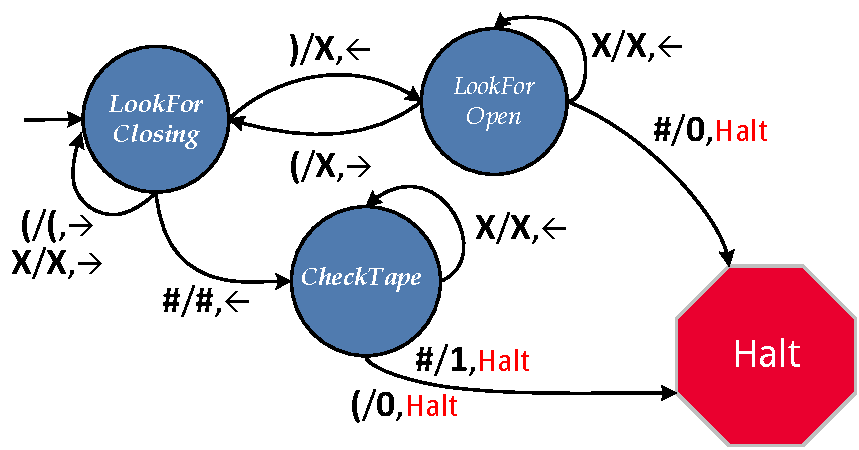
\includegraphics[width=4.5in]{figures/tm-parens.pdf}
\caption{Checking parentheses Turing Machine.\label{fig:tm-parens}}
\end{center} 
\end{figure}

\beforeex
\begin{exercise}
Follow the rules to simulate the checking parentheses Turing Machine on each input (assume the beginning and end of the input are marked with a \hash):
\begin{subexerciselist}
\item \tmtext{)}
\solution{

The descriptions below reference the rules from Figure~6.5. Assume the rules are numbered
from top to bottom starting with 1. In all use cases below, the machine starts in
\emph{LookForClosing} state, the head is above the start symbol \tmtext{\#}, and it moves to the right one
square.

To process \tmtext{)} we use rules 1 (\emph{Found closing}) and 8 (\emph{Reached beginning}, Halt).
}


%\item \tmtext{(}
\item \tmtext{()}
\solution{
2, 1, 6, 3, 4, 11, 11, 12.
}

\item \emph{empty input}
\solution{
4, 12.
}

\item \tmtext{(()(()))()}
\solution{
2, 2, 1, 6, 3, 2, 2, 1, 6, 3, 1, 7, 7, 6, 3, 3, 3, 1, 7, 7, 7, 7, 7, 7, 6, 3, 3, 3, 3, 3, 3, 3, 2, 1,
6, 3, 4, 11, 11, 11, 11, 11, 11, 11, 11, 11, 11, 12.
}
\item \tmtext{(()))(()}
\solution{
2, 2, 1, 6, 3, 1, 7, 7, 6, 3, 3, 3, 1, 7, 7, 7, 7, 8.
}
\end{subexerciselist}
\end{exercise}
\afterex
\end{examplenobar}

\beforeex
\begin{exercise} \goldstar 
Design a Turing Machine for adding two arbitrary-length binary numbers.  The input is of the form $a_{n-1} \ldots a_1 a_0$ \tmtext{+} $b_{m-1} \ldots b_1 b_0$ (with \hash\ markers at both ends) where each $a_k$ and $b_k$ is either \tmtext{0} or \tmtext{1}.  The output tape should contain bits that represent the sum of the two inputs.
\solution{

There are many strategies that can work for this, but its best to break the problem into a few subtasks like finding the least significant remaining digit, adding two bits (with a stored carry in the state), moving to the next position for writing the output, etc. For a problem this complicated, there are many on-line Turing Machine simulators to use to develop and test your solution.

}
\end{exercise}
\afterex

\splitbio{Alan Turing}{\index{people}{Turing, Alan}\index{general}{Entscheidungsproblem}\index{people}{Hilbert, David}
Alan Turing was born in London in 1912, and developed his computing model while at Cambridge in the 1930s. He developed the model to solve a famous problem posed by David Hilbert in 1928.  
The problem, known as the \emph{Entscheidungsproblem} (German for ``decision problem'') asked for an algorithm that could determine the truth or falsehood of a mathematical statement.  To solve the problem, Turing first needed a formal model of an algorithm.  For this, he invented the Turing Machine model described above, and defined an algorithm as any Turing Machine that is guaranteed to eventually halt on any input.  \sidepicture{0.22}{images/Turing2.jpg}{Alan Turing}{Image from Bletchley Park Ltd.} 
% http://www.bletchleypark.org.uk/doc/image.rhtm/Turing2.jpg
With the model, Turing was able to show that there are some problems that cannot be solved by \emph{any} algorithm.  We return to this in Chapter~\ref{ch:computability} and explain Turing's proof and examples of problems that cannot be solved.

\index{people}{Church, Alonzo}\index{general}{Lambda calculus}\index{general}{Enigma}\index{general}{Bletchley Park}After publishing his solution to the \emph{Entscheidungsproblem} in 1936, Turing went to Princeton and studied with Alonzo Church (inventor of the Lambda calculus, on which Scheme is based).  With the start of World War II, Turing joined the highly secret British effort to break Nazi codes at Bletchley Park.  Turing was instrumental in breaking the Enigma code which was used by the Nazis to communicate with field units and submarines.  Turing designed an electro-mechanical machine known as a \emph{bombe} for searching possible keys to decrypt Enigma-encrypted messages.  
\sidepicture{0.028}{images/edit/bletchley-bombe-P1010122.jpg}{Bombe}{Rebuilt at Bletchley Park}
The machines used logical operations to search the possible rotor settings on the Enigma to find the settings that were most likely to have generated an intercepted encrypted message. Bletchley Park was able to break thousands of Enigma messages during the war.  The Allies used the knowledge gained from them to avoid Nazi submarines and gain a tremendous tactical advantage.
 
After the war, Turing continued to make both practical and theoretical contributions to computer science.  Among other things, he worked on designing general-purpose computing machines and published a paper (\emph{Intelligent Machinery}) speculating on the ability of computers to exhibit intelligence.  Turing introduced a test for machine intelligence (now known as the Turing Test) based on a machines ability to impersonate a human and speculated that machines would be able to pass the test within 50 years (that is, by the year 2000).  Turing also studied morphogenesis (how biological systems grow) including why Fibonacci numbers appear so often in plants.

In 1952, Turing's house was broken into, and Turing reported the crime to the police.  The investigation revealed that Turing was a homosexual, which at the time was considered a crime in Britain.  Turing did not attempt to hide his homosexuality, and was convicted and given a choice between serving time in prison and taking hormone treatments. He accepted the treatments, and has his security clearance revoked.  In 1954, at the age of 41, Turing was found dead in an apparent suicide, with a cyanide-laced partially-eaten apple next to him.  The codebreaking effort at Bletchley Park was kept secret for many years after the war (Turing's report on Enigma was not declassified until 1996), so Turing never received public recognition for his contributions to the war effort.  In September 2009, instigated by an on-line petition, British Prime Minister Gordon Brown issued an apology for how the British government treated Alan Turing.\index{people}{Brown, Gordon}
}

%\ex{\goldstar Suppose we need to balance curly brackets as well as parentheses.  For example, \verb|{()}| is well-balanced, but \verb|{(})| is not.  Devise a Turing Machine that outputs \tmtext{1} when its input is a well-balanced string of parentheses and square brackets, and outputs \tmtext{0} otherwise.  Use as few states as possible.}


\LATER{
\begin{example}{Adding Machine}

\end{example}

\begin{example}{Multi-Tape Machines}

\end{example}

\section{Universal Computers}\label{sec:universal}
}

\section{Summary}

The power of computers comes from their programmability.  Universal computers can be programmed to execute any algorithm.  The Turing Machine model provides a simple, abstract, model of a computing machine.  Every algorithm can be implemented as a Turing Machine, and a Turing Machine can simulate any other reasonable computer.

As the first computer programmer, Ada deserves the last word:\index{people}{Ada, Countess of Lovelace}
\begin{smallquote}{\em
%It may be desirable to explain, that 
By the word operation, we mean any process which alters the mutual relation of two or more things, be this relation of what kind it may. This is the most general definition, and would include all subjects in the universe. In abstract mathematics, of course operations alter those particular relations which are involved in the considerations of number and space, and the results of operations are those peculiar results which correspond to the nature of the subjects of operation. But the science of operations, as derived from mathematics more especially, is a science of itself, and has its own abstract truth and value; just as logic has its own peculiar truth and value, independently of the subjects to which we may apply its reasonings and processes.$\ldots$

The operating mechanism can even be thrown into action independently of any object to operate upon (although of course no result could then be developed). Again, it might act upon other things besides number, were objects found whose mutual fundamental relations could be expressed by those of the abstract science of operations, and which should be also susceptible of adaptations to the action of the operating notation and mechanism of the engine. Supposing, for instance, that the fundamental relations of pitched sounds in the science of harmony and of musical composition were susceptible of such expression and adaptations, the engine might compose elaborate and scientific pieces of music of any degree of complexity or extent. }

\raggedleft Ada, Countess of Lovelace, \emph{Sketch of The Analytical Engine}, \cut{Translator's Note A,} 1843 %http://www.fourmilab.ch/babbage/sketch.html
\index{general}{Analytical Engine}
\end{smallquote} 

\end{schemeregion}
